\documentclass[twocolumn,a4paper,dvipdfmx]{ieicejsp}
\usepackage[T1]{fontenc}
\usepackage{lmodern}
\usepackage{textcomp}
\usepackage{latexsym}
\usepackage{float}
\usepackage{graphicx}
\usepackage{amsmath, amssymb}
\usepackage{bm}
\usepackage{upgreek}
\usepackage{caption}
\usepackage{booktabs}
\usepackage{multirow}
\usepackage{array}
\usepackage{tikz}
\usetikzlibrary{positioning, arrows.meta, fit}

\captionsetup{font=small}
\setlength{\floatsep}{12pt plus 2pt minus 2pt}
\setlength{\textfloatsep}{14pt plus 2pt minus 2pt}
\setlength{\dblfloatsep}{12pt plus 2pt minus 2pt}
\setlength{\dbltextfloatsep}{14pt plus 2pt minus 2pt}
\setlength{\intextsep}{12pt plus 2pt minus 2pt}

\title{
    {\bf 視覚言語モデルからの知識蒸留による大喜利お題画像の大規模アノテーション}
    {\normalsize \\ Large-Scale Annotation of Ogiri Prompt Images via Knowledge Distillation from a Vision-Language Model}
}
\author{
    山富 龍 \\ Ryo Yamatomi
}
\affliate{%
    湘南工科大学 大学院 \\
    Graduate University of Shonan Institute of Technology\\
}

\begin{document}
\maketitle
\thispagestyle{plain}
\pagestyle{plain}

\begin{abstract}
大喜利投稿サイト「ボケて」では，投稿者が掲示した画像（お題画像）に対して利用者が面白い一言（ボケ）を投稿する．
お題画像には，通常の写真のほかに，空欄に入る語を答える穴埋め，ひらがなから始まる文を作るカルタ，画像中の問いに答えるお題文などの形式があり，形式ごとにボケの生成に必要な処理が異なる．
本稿では，ボケてから収集した約682万件のお題画像に対し，大喜利の形式，画像中の記号や文字の有無，画像の媒体を表すラベルを，有料の API を用いずに単一の GPU で付与する方法を確立するまでの経緯と分析を報告する．
まず，ゼロショット分類，メタデータを用いた弱教師あり学習，視覚言語モデル (Vision-Language Model，VLM) による直接の分類，VLM のラベルを高速な画像分類器に移す知識蒸留を比較し，VLM である Qwen3-VL-8B を教師とし，SigLIP 2 の画像埋め込みに基づく分類器を生徒とする蒸留が，教師と同等以上の精度を約1桁速い速度で得ることを示した．
次に，精度の上限がラベルの定義の曖昧さによって決まっていることを示し，ボケの生成に必要な処理から逆算してラベルの定義を4回改訂した．
さらに，VLM への質問を軸ごとに分割する方法，誤りやすいクラスに限って別の短い質問で確かめる方法，少ない区分の画像を生徒の予測で選んで追加する方法，2種類の生徒の確率を平均する方法を導入した．
最終の構成は，目視のラベルに対して，評価用データで3軸のマクロ F1 の平均 0.919，実データで全項目が一致する画像の割合の推定値 0.838 を達成し，全データの予測を約10.2時間で完了した．
\par
\noindent
{\bf キーワード} 大喜利，データアノテーション，視覚言語モデル，知識蒸留，ラベル設計
\end{abstract}

\section*{Abstract}
On the Japanese comedy site Bokete, users post a witty line (boke) in response to a prompt image (odai).
Prompt images come in several formats, such as fill-in-the-blank images, karuta cards that require a line starting with a given hiragana character, and images containing a written question, and each format requires a different generation process.
This paper reports how we established a method to annotate about 6.82 million prompt images with their Ogiri format, the presence of symbols and text, and the visual medium, on a single GPU without paid APIs.
We first compare zero-shot classification, weak supervision from metadata, direct classification by a vision-language model (VLM), and knowledge distillation, and show that distilling labels of Qwen3-VL-8B into classifiers on SigLIP 2 embeddings matches the teacher's accuracy at roughly ten times its speed.
We then show that the accuracy is bounded by ambiguity in the label definitions, and revise the definitions four times by deriving them from the processes needed to generate a boke.
We further introduce axis-wise questioning of the VLM, a separate verification question for error-prone classes, mining of rare classes with student predictions, and averaging the probabilities of two students.
The final pipeline achieves an average macro F1 of 0.919 over three axes on the evaluation set and an estimated exact-match rate of 0.838 on real data, and predicts all images in about 10.2 hours.
\par
\noindent
{\bf Key words} Ogiri, Data Annotation, Vision-Language Model, Knowledge Distillation, Label Design

\section{はじめに}
大喜利は，出題された題目に対して機知に富んだ回答を返す言葉遊びであり，ユーモアの生成と理解を扱う研究の題材として用いられている．
大喜利投稿サイト「ボケて」\cite{ref_bokete}では，投稿者がお題となる画像を掲示し，他の利用者がその画像に対する面白い一言を投稿する．
ボケてに蓄積された画像と回答の組は，画像を入力として面白い文を生成するモデルの学習や，ユーモアの分析に利用できる大規模な資源である．
本稿では，ボケてから収集したデータベースを，学習や分析に用いやすい形に整えるため，全てのお題画像に種類を表すラベルを付与する作業を扱う．
以下では，データにラベルを付与する作業をアノテーションと呼ぶ．

お題画像には，現実の写真のように画像を見て一言を付ければよいものだけでなく，回答の形を制限するものがある．
例えば，画像中の空欄に入る語を答える穴埋め，画像の隅に書かれたひらがな1文字から始まる文を作るカルタ，画像に書かれた問いや指示に答えるお題文がある．
また，アニメのスクリーンショットや漫画のコマのように，作品の知識を前提とする画像もある．
これらの画像からボケを生成するには，空欄の位置の検出，ひらがなの読み取り，文字の読み取りなど，種類ごとに異なる処理が必要になる．
したがって，生成モデルの学習やデータの分析では，各お題画像がどの種類に属するかを事前に知る必要がある．

アノテーションの対象は約682万件のお題画像であり，人手で全てにラベルを付けることは現実的ではない．
近年の視覚言語モデル (Vision-Language Model，VLM) は，画像と指示文を入力として，指示に従った分類を学習なしで行える．
しかし，有料の API で約682万件を処理すると費用が大きく，ローカルの GPU で VLM を全件に適用しても約70時間以上を要する．
さらに，ラベルの定義を見直すたびに全件を処理し直す必要がある．
そこで本稿では，有料の API を用いず，単一の GPU で全件を現実的な時間で処理できるアノテーションの方法を確立することを目的とする．

本研究は，方法の比較，ラベルの定義の改訂，評価の厳密化を繰り返す試行錯誤の過程を経て，最終の方法に到達した．
本稿では，最終の方法だけでなく，その過程で得られた知見を，以下の観点からまとめる．
\begin{itemize}
    \item ゼロショット分類，メタデータによる弱教師あり学習，VLM による直接の分類，VLM のラベルを高速な分類器に移す知識蒸留を比較し，蒸留が精度と速度の両面で最良であることを示す．
    \item 強い手法に共通する誤りの多くがラベルの定義の境界にあることを示し，ボケの生成に必要な処理から逆算してラベルの定義を改訂する過程と，その各段階での判断の根拠を示す．
    \item VLM への指示の方法について，質問を分割する方法，説明を書き足す方法，別の短い質問で確かめる方法などの成否を比較し，有効であった方法とそうでなかった方法の傾向を示す．
    \item 出現率の低い区分を扱うための学習データの追加，重み付きの損失，複数の分類器の確率の平均を比較し，最終の構成を決める．
    \item 最終の構成を全データに適用し，ラベルの分布と投稿年ごとの推移を示す．
\end{itemize}

本稿の構成は次のとおりである．
\ref{sec_data}章で対象のデータと本稿で用いる用語を定義し，\ref{sec_related}章で関連する技術を整理する．
\ref{sec_eval}章で評価用データと評価指標を定義する．
\ref{sec_selection}章で手法の選定の実験を述べ，\ref{sec_label}章でラベルの定義の改訂の経緯を述べる．
\ref{sec_teacher}章と\ref{sec_student}章で，教師となる VLM への指示の方法と，生徒となる分類器の構成をそれぞれ検討する．
\ref{sec_final}章で最終の構成とその精度を示し，\ref{sec_full}章で全データへの適用の結果を示す．
\ref{sec_discussion}章で得られた知見と限界を考察し，\ref{sec_conclusion}章でまとめる．

\section{対象データと用語}
\label{sec_data}
\subsection{ボケてとお題画像}
ボケてでは，投稿者が1枚の画像を掲示し，その画像を題目とする大喜利の場を作る．
本稿では，この画像をお題画像と呼び，お題画像とその投稿の単位をお題と呼ぶ．
他の利用者がお題に対して投稿する面白い一言をボケと呼ぶ．
各お題は数値の識別子（お題 ID）を持ち，1件のお題には0件以上のボケが付く．

本稿で用いるデータは，ボケてから収集した1次データからなるデータベース BoketeDBv4 である．
BoketeDBv4 は，お題，ボケ，お題画像，利用者，評価などの表からなり，各表は Apache Parquet 形式で保存されている．
お題画像の表は6,823,270件の画像を含み，各画像のファイルの内容から求めた SHA-256 のハッシュ値を持つ．
ハッシュ値が同じ画像は内容が同一であり，同一の内容をまとめると6,609,511枚となる．
お題の投稿年は2008年から2026年にわたり，2014年から2023年に毎年40万件以上が投稿されている．

お題の表には，投稿者が投稿時に選んだ画像の種類を表す \texttt{type} 列がある．
\texttt{type} 列は2022年以降の約80万件のお題にのみ値があり，値は「写真」「イラスト」「穴埋め」「文字」「その他」のいずれかである．
また，お題には投稿者や閲覧者が付けたタグがあり，「穴埋め」「かるた」「漫画」「アニメ」などのタグを含む．
これらのメタデータは画像の種類の手がかりになるが，\ref{sec_selection}章で示すとおり，ラベルとして用いるには誤りが多い．

\subsection{お題画像の種類と処理の要件}
お題画像の種類のうち，ボケの生成の処理に影響するものは次のとおりである．
現実画像は，現実の写真であり，画像の内容を見て一言を付ければよい．
アニメのスクリーンショットと漫画のコマの切り抜きは，その画像のキャラクターや作品の知識を前提とすることがある．
文章のお題が書かれた画像は，画像中の文字を読み取ったうえで，その文章に答える必要がある．
穴埋め画像は，画像中に矩形や円などの空欄の記号があり，利用者はその空欄に入る語をボケとして投稿する．
例えば「東京大学○○学部」の画像では，○○に入る語を答える．
カルタ画像は，画像中の円などの記号の中にひらがな1文字が書かれており，利用者はそのひらがなから始まる文を投稿する．
穴埋めとカルタでは，記号の位置やひらがなを検出したうえでボケを生成する必要がある．

これらの種類を約682万件のお題画像に付与する処理には，次の要件がある．
第1に，有料の API を用いず，ローカルの計算機で処理する．
第2に，全件の処理を現実的な時間，具体的には単一の GPU で1日程度以内に終える．
第3に，ラベルの定義を見直した場合に，全件の処理をやり直す費用が小さい．
本研究の実験は全て，VRAM が96GB の NVIDIA RTX PRO 6000 Blackwell を1基備えた計算機で行った．

\subsection{本稿で用いる用語}
本稿では，ラベルの構成や処理の構成を表すために，いくつかの用語を独自の意味で用いる．
表\ref{tab_terms}に，主な用語とその意味をまとめる．
各用語は，初めて用いる箇所でも改めて説明する．

\begin{table*}[t]
    \centering
    \caption{本稿で用いる主な用語}
    \label{tab_terms}
    \small
    \begin{tabular}{>{\raggedright\arraybackslash}p{0.2\textwidth}>{\raggedright\arraybackslash}p{0.74\textwidth}}
        \toprule
        用語 & 意味 \\
        \midrule
        形式 & 大喜利の回答の形を制限するお題画像の性質．カルタ，穴埋め，お題文，通常の4クラスから1つを選ぶ \\
        お題文 & 投稿者が画像に書き加えた，回答者に向けた問い，指示，題目の句などの文．形式のクラス名としても用いる \\
        属性 & 形式とは独立に，画像中の記号や文字の有無を表す複数選択のラベル．最終の定義では空欄あり，カルタ記号あり，文字ありの3項目 \\
        媒体 & 画像の画風や由来を表すラベル．写真，アニメ，ゲーム，マンガ，テキストグラフィック，絵画，イラストの7クラスから原則1つを選ぶ \\
        軸 & 形式，属性，媒体のように，独立に判定するラベルのまとまり \\
        定義書 & ラベルの定義を文章でまとめた文書．第1版から第4版まで改訂した \\
        教師 & 学習用のラベルを付ける VLM．本稿では Qwen3-VL-8B に複数の質問をする構成全体を指す \\
        教師ラベル & 教師が画像に付けたラベル．生徒の学習に用いる \\
        生徒 & 教師ラベルで学習し，全件の処理に用いる高速な画像分類器 \\
        蒸留 & 教師の判断を，教師ラベルを用いた学習によって生徒に移すこと \\
        目視ラベル & 判断者が画像を見て付けたラベル．評価にのみ用いる \\
        通常の評価用データ & 目視ラベルを付けた640枚の評価用の画像．調整用（dev）と最終評価用（test）に二分する \\
        少ない区分 & 出現率が数\%以下のクラス．具体的にはゲーム，CG，絵画，カルタ \\
        少ない区分の評価用データ & 少ない区分を多く含むように抽出し，目視ラベルを付けた800枚の評価用の画像 \\
        実データの目視ラベル & 学習にも評価用データにも用いていない画像から抽出し，目視ラベルを付けた380枚．無作為抽出の160枚と層別抽出の220枚からなる \\
        少ない区分の追加 & 生徒の予測で少ない区分らしい画像を選び，教師ラベルを付けて学習データに加えること \\
        確認の質問 & 生徒または教師がお題文と判定した画像に限り，VLM に別の短い質問をして判定を確かめる処理 \\
        書き出しの集中度 & お題に付いたボケの最初の文字が，最も多い1文字に集中している割合．カルタの判定の補助に用いる \\
        全項目一致 & 形式，属性，媒体の全ての項目が目視ラベルと一致した画像の割合 \\
        \bottomrule
    \end{tabular}
\end{table*}

\section{関連技術}
\label{sec_related}
本章では，本研究で比較した手法の基礎となる技術を整理する．

\subsection{画像とテキストの埋め込みモデル}
Contrastive Language-Image Pre-training (CLIP)\cite{ref_clip} は，画像と文章を同じベクトル空間に写す2つのエンコーダを，大量の画像と説明文の組から対照学習したモデルである．
以下では，エンコーダが出力するベクトルを埋め込みと呼ぶ．
SigLIP\cite{ref_siglip} は，CLIP の対照学習の損失をシグモイド関数による2値の損失に置き換えたモデルであり，SigLIP 2\cite{ref_siglip2} は多言語の学習データや位置の情報を扱う学習を加えた後継のモデルである．
本研究では，CLIP の ViT-B/32 のモデル（以下，CLIP-B/32），入力が224画素の SigLIP 2 の Base のモデル（以下，SigLIP2-B），入力が384画素の SigLIP 2 の so400m のモデル（以下，SigLIP2-so400m）を用いた．

埋め込みモデルによる分類には2通りの使い方がある．
1つ目はゼロショット分類であり，各クラスを表す文章の埋め込みと画像の埋め込みのコサイン類似度が最大のクラスを選ぶ．
学習データは不要であるが，分類の精度は文章の選び方に依存する．
2つ目は，画像の埋め込みを特徴量とし，ラベル付きのデータでロジスティック回帰などの分類器を学習する方法である．
特に線形の分類器を用いる場合を線形プローブと呼ぶ．
いずれも1枚あたりの計算量は画像エンコーダの1回の順伝播のみであり，GPU で毎秒数百から千枚程度を処理できる．

\subsection{視覚言語モデル}
VLM は，画像と指示文を入力として文章を生成するモデルである．
クラスの定義を自然言語で与えるだけで分類でき，学習データを必要としない．
本研究では，Qwen3-VL\cite{ref_qwen3vl} の Instruct のモデルを主に用い，比較として InternVL3.5\cite{ref_internvl35} と MiniCPM-V 4.5\cite{ref_minicpmv} を用いた．
推論には，大規模言語モデルの推論を高速化するライブラリ vLLM\cite{ref_vllm} を用いた．
vLLM の構造化出力の機能を用いると，出力を JSON スキーマや正規表現に一致する文字列に制約できる．
本研究では全ての VLM の出力をラベルの候補に制約したため，出力を解釈できない事例は生じなかった．
VLM は精度が高い一方で，1枚あたりの計算量が埋め込みモデルより1桁以上大きく，Qwen3-VL-8B で毎秒25枚程度であった．

\subsection{知識蒸留}
知識蒸留\cite{ref_kd}は，大きく高精度なモデル（教師）の出力を目標として，小さく高速なモデル（生徒）を学習する方法である．
本研究では，教師である VLM が一部の画像に付けたラベルを正解として，埋め込みに基づく分類器や画像エンコーダを学習する．
教師が全件を処理する代わりに，教師は数万枚にラベルを付けるのみであり，全件の処理は高速な生徒が行う．
また，埋め込みを一度計算して保存しておけば，ラベルの定義を変えた場合も，教師ラベルを付け直して小さな分類器を再学習するだけで全件のラベルを更新できる．

\subsection{画像エンコーダの微調整}
埋め込みを固定して分類器のみを学習する代わりに，画像エンコーダ全体を教師ラベルで追加学習することもできる．
以下では，これを微調整と呼ぶ．
微調整は，埋め込みに基づく分類器より多くの計算を学習時に要するが，小さな画像エンコーダでも大きなモデルの埋め込みに近い精度を得られる場合がある．
本研究では，SigLIP2-B と ConvNeXt-Tiny\cite{ref_convnext} の微調整を比較した．

\section{評価の枠組み}
\label{sec_eval}
本研究では，手法やラベルの定義の改訂に合わせて評価用データを拡充してきた．
本章では，最終的に用いた3種類の評価用データと評価指標を定義し，それぞれを導入した理由を述べる．

\subsection{目視ラベルの付与}
評価に用いる正解のラベルは，判断者が画像を1枚ずつ見て付与した．
以下では，このラベルを目視ラベルと呼ぶ．
目視ラベルの付与は，画像を表示して内容を確認できる AI エージェントである Claude Code が，その時点の定義書に従って行った．
付与の際は，画像を20枚ずつ並べた一覧画像を作成し，各画像に番号とお題 ID を表示した．
評価する手法の予測は一覧画像に表示せず，予測に判断が引きずられないようにした．
目視ラベルは全て1名の判断者によるものであり，判断者間の一致度は測っていない．
この点は本研究の限界であり，\ref{sec_discussion}章で改めて述べる．

\subsection{通常の評価用データ}
通常の評価用データは，全てのお題から無作為に抽出した440枚と，少ない種類を補うためにメタデータで絞り込んだ200枚の計640枚からなる．
メタデータによる絞り込みでは，\texttt{type} 列が穴埋め，文字，イラストのお題と，カルタ，漫画，アニメのタグが付いたお題から抽出した．
最初の実験では440枚であり，2回目の実験で無作為抽出の200枚を加えて640枚とした．
目視ラベルは，ラベルの定義を改訂するたびに付け直した．

プロンプトの改訂を評価用データの誤りを見ながら行うと，評価用データでの精度は楽観的になる．
そこで，3軸のラベルを導入した段階から，640枚を形式で層化して320枚ずつに二分した．
以下では，プロンプトや構成の選択に用いる半分を調整用データ（dev），最終的な精度の報告にのみ用いる半分を最終評価用データ（test）と呼ぶ．
また，生徒のハイパーパラメータは，評価用データではなく，教師ラベルの一部を取り分けた検証用分割で選んだ．

\subsection{少ない区分の評価用データ}
通常の評価用データには，出現率の低いクラスがほとんど含まれない．
例えば，絵画は640枚中5枚，CG は4枚であり，1枚の正誤で F1 が大きく変わる．
そこで，ゲーム，CG，絵画，カルタの4区分を多く含む評価用データを別に作成した．
以下では，出現率が数\%以下のこれらのクラスを少ない区分と呼ぶ．

第1版は，生徒が各区分である確率の上位2,000枚から，区分ごとに50枚を無作為に抽出した200枚である．
第2版では，学習にも評価にも用いていない294,802枚の画像に生徒の確率を付け，区分 $ c $ ごとに確率が0.5以上の層と，0.05以上0.5未満の層から60枚ずつを抽出した．
さらに全体から無作為に120枚を加え，計600枚とした．
第1版と第2版を合わせた800枚を，抽出の層ごとに dev と test に二分した．
この評価用データは確率で絞り込んだ画像からなるため，区分の出現率は実際より高い．
したがって，このデータでの値は手法間の比較にのみ用いる．

\subsection{実データの目視ラベル}
通常の評価用データには，ボケての典型的な画像の一部が少ないことが，研究の後半で明らかになった．
そこで，学習にも評価用データにも用いていない実データから，2通りの方法で画像を抽出し，目視ラベルを付けた．
1つ目は無作為抽出の160枚であり，実際の分布での精度を直接表す．
2つ目は層別抽出の220枚である．
層別抽出では，生徒が予測したクラスのうち実データで最も出現率の低いものを各画像の層とし，11の層から20枚ずつを抽出した．
これにより，絵画，カルタ，ゲーム，お題文などの少ないクラスを各15枚から20枚程度確保した．
無作為抽出と層別抽出を合わせて，実データの目視ラベルと呼ぶ．

層別抽出の画像は抽出の確率が層によって異なるため，単純に集計すると少ないクラスの影響が過大になる．
そこで，各画像に抽出確率の逆数の重みを付けて，実際の分布での精度を推定した．
画像 $ i $ の重み $ w_i $ と，ある指標の推定値 $ \hat{\mu} $ を(\ref{eq_ipw})に示す．

\begin{equation}
    w_i = \frac{N_{h(i)}}{n_{h(i)}},
    \qquad
    \hat{\mu} = \frac{\sum_{i} w_i z_i}{\sum_{i} w_i}
    \label{eq_ipw}
\end{equation}

\noindent
ここで $ h(i) $ が画像 $ i $ の層，$ N_h $ が実データ294,802枚のうち層 $ h $ に属する画像の数，$ n_h $ が層 $ h $ から抽出した画像の数，$ z_i \in \{0, 1\} $ が画像 $ i $ で指標の条件が成り立つかを表す値である．
無作為抽出の160枚は，全体の画像数を抽出数で割った重みで同じ式に加えた．
以下では，この値を推定値と呼ぶ．

\subsection{評価指標}
形式のように1つのクラスを選ぶ軸は，正解率とマクロ F1 で評価した．
マクロ F1 を(\ref{eq_macro_f1})に示す．

\begin{equation}
    {\rm F1}_{\rm macro} = \frac{1}{K} \sum_{k=1}^{K} \frac{2 P_k R_k}{P_k + R_k}
    \label{eq_macro_f1}
\end{equation}

\noindent
ここで $ K $ がクラス数，$ P_k $ と $ R_k $ がクラス $ k $ の適合率と再現率である．
マクロ F1 は，件数の少ないクラスの性能を件数の多いクラスと等しく反映する．
属性と媒体のように複数の項目を選びうる軸は，項目ごとに2値分類の F1 を求め，評価用データに正例がある項目の F1 を平均して，その軸のマクロ F1 とした．
総合の指標として，形式，属性，媒体の3軸のマクロ F1 の平均を用い，以下では3軸の平均と呼ぶ．

件数の少ない項目は F1 の推定が不安定であるため，正例が10件以上ある項目のみで求めた平均も併用し，頑健な指標と呼ぶ．
少ない区分の評価用データでは，各区分の F1 の平均を用いた．
実データの目視ラベルでは，全ての項目が目視ラベルと一致した画像の割合を全項目一致と呼び，(\ref{eq_ipw})による推定値を主な指標とした．
2つの構成の全項目一致の差の信頼区間は，画像を単位とする対応のある自助法により，2,000回の再標本化で求めた．

\section{手法の選定}
\label{sec_selection}
本章では，研究の初期に行った手法の比較を述べる．
この段階では，ラベルを単純な7クラスとし，ラベルの付け方そのものを比較した．

\subsection{初期のラベル}
初期のラベルは，ボケの生成の処理を決める形式と，事前知識の要否を決める画風の2つの軸で定義した．
形式は，主となる絵や写真がなく画像の大部分が文章である text，空欄の記号がある anaume，カルタの札の形式である karuta，それ以外の normal の4値とした．
画風は，写真 photo，アニメ anime，漫画 manga，その他の絵 illust の4値とした．
比較には，形式が normal 以外なら形式を，normal なら画風を採る7クラス（photo，anime，manga，text，anaume，karuta，illust）を用いた．
無作為抽出の440枚の目視ラベルでは，photo が44.5\%，anaume が22.3\%，illust が9.3\%，text が8.6\%，manga が7.0\%，anime が6.6\%，karuta が1.6\%であった．
穴埋めはお題の約4分の1を占め，最も多い特殊な形式である．

\subsection{比較した手法}
比較した手法は次の5系統である．
1つ目は，埋め込みモデルのゼロショット分類であり，各クラスに3個から4個の英語の文章を用意した．
2つ目は，メタデータを弱いラベルとした線形プローブである．
\texttt{type} 列とタグから各クラス1,500枚，計10,500枚を抽出し，その値をラベルとした．
3つ目は，Qwen3-VL の 2B，4B，8B の各モデルに，画像と2つの軸の定義を与えて直接分類させる方法である．
4つ目は，Qwen3-VL が10,500枚に付けたラベルで線形プローブを学習する蒸留である．
5つ目は，日本語の文字認識 (Optical Character Recognition，OCR) のライブラリ YomiToku\cite{ref_yomitoku} で文字の領域を検出し，文字の面積比と文字数が大きい画像を text とする規則である．
線形プローブは，標準化した埋め込みに対する L2 正則化付きのロジスティック回帰とした．

\subsection{初期の比較の結果}
図\ref{fig_speed_vs_f1}に，評価用データ440枚における各手法の処理速度と7クラスのマクロ F1 を示す．
横軸は1秒あたりの処理枚数，上側の横軸は全件の処理に要する時間であり，いずれも対数軸である．
図中の vlm は VLM による直接の分類，probe\_vlm は VLM のラベルによる蒸留，probe\_hand は目視ラベルによる線形プローブ，probe\_weak はメタデータの弱いラベルによる線形プローブ，zeroshot はゼロショット分類を表す．

\begin{figure}[t]
    \centering
    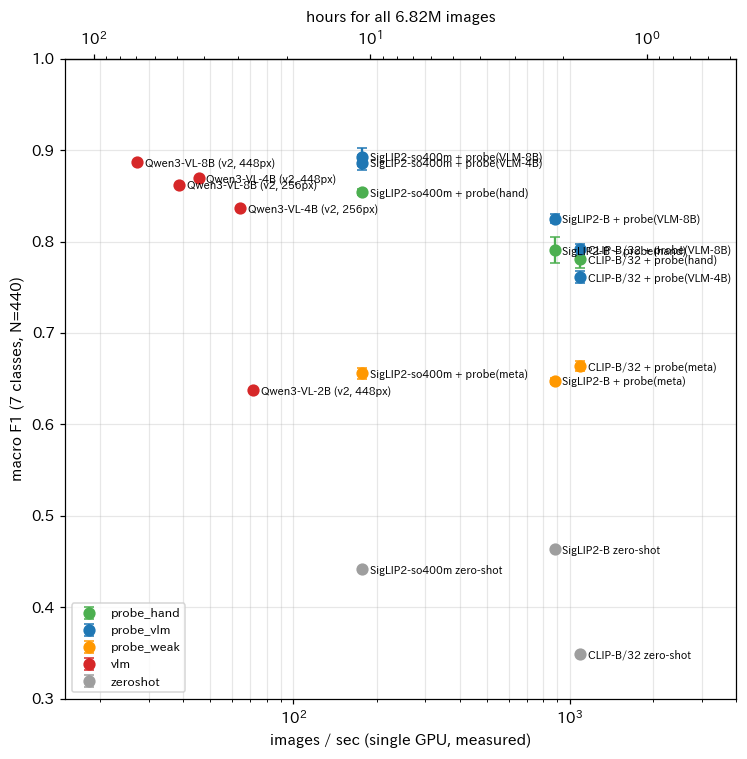
\includegraphics[width=\linewidth]{figures/fig_speed_vs_f1.png}
    \caption{初期のラベルにおける各手法の処理速度と7クラスのマクロ F1}
    \label{fig_speed_vs_f1}
\end{figure}

ゼロショット分類のマクロ F1 は 0.35 から 0.46 にとどまり，穴埋めの120枚のうち77枚を normal と予測した．
空欄があるという画像の部分的な特徴は，画像全体と文章の類似度では捉えにくい．
メタデータを弱いラベルとした学習は，正解率が約0.70にとどまった．
漫画のタグが付いた30枚のうち16枚が穴埋めであったように，メタデータは画像の種類と1対1に対応しないためである．
OCR の規則は，形式の正解率が 0.568 で，処理速度も毎秒6.4枚と遅かった．

Qwen3-VL-8B による直接の分類は正解率 0.905 であったが，処理速度は毎秒約27枚であり，全件に約70時間を要する．
このとき，プロンプトの text の定義を「画像の大部分が文章であり，主となる写真や絵がない」に限定し，字幕や看板を含む画像は normal とする記述を加えると，正解率は 0.718 から 0.905 に向上した．
限定する前のプロンプトでは，normal の219枚のうち98枚を text と予測していた．
モデルの大きさを変えるより，プロンプトの定義を明確にする効果の方が大きかった．

Qwen3-VL-8B のラベルで学習した SigLIP2-so400m の線形プローブは，正解率 0.913，マクロ F1 0.893 であり，教師と同等以上の精度を教師の約6.5倍の速度で得た．この生徒の速度は毎秒178枚であり，全件を約10.7時間で処理できる．
目視ラベル440枚で学習した線形プローブの正解率は 0.882 であり，VLM の約9,500枚のラベルによる学習に及ばなかった．
一方，教師を Qwen3-VL-2B にすると生徒の正解率は 0.726 にとどまり，教師の精度が生徒の精度の上限をおおむね決めていた．
これらの結果から，精度を決めるのはモデルの大きさよりもラベルの質であり，VLM の判断を高速な分類器に移す蒸留が有望であると判断した．

\subsection{蒸留の構成要素の比較}
次に，蒸留を構成する要素を1つずつ入れ替えて比較した．
この実験から，評価用データを640枚に拡充し，ハイパーパラメータを教師ラベルの検証用分割で選ぶようにした．
教師ラベル用の画像として，全てのお題から無作為に40,000枚を抽出し，学習用36,000枚と検証用4,000枚に分けた．
表\ref{tab_distill_components}に主な結果を示す．

\begin{table}[t]
    \centering
    \caption{蒸留の構成要素の比較（評価用データ640枚，7クラスの正解率）}
    \label{tab_distill_components}
    \small
    \begin{tabular}{lcc}
        \toprule
        手法 & 正解率 & 全件の時間 \\
        \midrule
        教師 Qwen3-VL-8B & 0.916 & 73 h \\
        教師 Qwen3-VL-32B（FP8） & 0.916 & 243 h \\
        教師 Qwen3-VL-30B-A3B（FP8） & 0.861 & 49 h \\
        教師 InternVL3.5-8B & 0.794 & 372 h \\
        教師 MiniCPM-V 4.5 & 0.684 & 143 h \\
        Qwen3-VL の3モデルの多数決 & 0.922 & -- \\
        \midrule
        LogReg，SigLIP2-so400m & 0.920 & 10.7 h \\
        MLP，SigLIP2-so400m & 0.911 & 10.7 h \\
        k 近傍法，SigLIP2-so400m & 0.811 & 10.7 h \\
        LogReg，SigLIP2-B & 0.867 & 2.2 h \\
        微調整 SigLIP2-B & 0.915 & 1.7 h \\
        微調整 ConvNeXt-Tiny & 0.902 & 2.7 h \\
        \bottomrule
    \end{tabular}
\end{table}

表\ref{tab_distill_components}の LogReg はロジスティック回帰，MLP は2層の多層パーセプトロン (Multi-Layer Perceptron，MLP) を表す．
生徒は全て Qwen3-VL-8B の教師ラベル36,000枚で学習し，3つの乱数の種の平均を示す．
教師は Qwen3-VL-8B が最良であった．
Qwen3-VL-32B は同じ正解率で約3.3倍遅く，30B-A3B と他系統の2モデルは穴埋めを過剰に検出する傾向があり，精度が劣った．
ただし，プロンプトは Qwen3-VL-8B の誤りを見て調整したものであり，他系統のモデルに不利な比較である可能性がある．
複数の教師の多数決は 8B 単体からの改善が0.6ポイントにとどまり，計算量に見合わなかった．

生徒では，ロジスティック回帰と MLP が同等であり，k 近傍法は件数の少ない karuta と雑多な illust で大きく劣った．
SigLIP2-B の微調整は，SigLIP2-B の埋め込みに対するロジスティック回帰より約5ポイント高く，SigLIP2-so400m の線形プローブと同等の精度を約6倍の速度で得た．
埋め込みの連結や，OpenCV で検出した空欄の矩形の特徴の追加による改善は0.005未満であり，強い埋め込みは空欄の情報を既に含んでいた．

図\ref{fig_learning_curve}に，教師ラベルの学習枚数と7クラスのマクロ F1 の関係を示す．
横軸は教師ラベルの学習枚数の対数，縦軸はマクロ F1 であり，実線は評価用データ，破線は教師ラベルの検証用分割での値である．
logreg はロジスティック回帰，mlp は MLP を表す．

\begin{figure}[t]
    \centering
    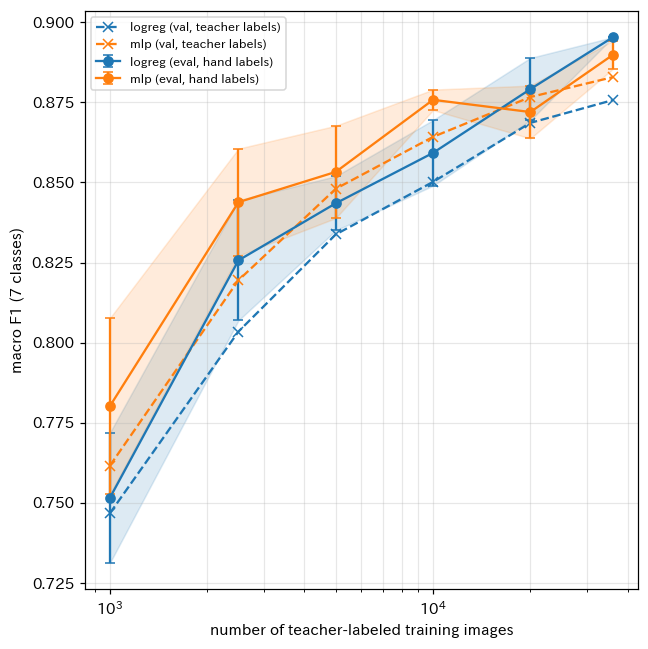
\includegraphics[width=0.9\linewidth]{figures/fig_learning_curve.png}
    \caption{教師ラベルの学習枚数とマクロ F1}
    \label{fig_learning_curve}
\end{figure}

マクロ F1 は学習枚数とともに単調に向上し，36,000枚でも飽和していなかった．
ロジスティック回帰の正解率は，1,000枚で 0.841，10,000枚で 0.891，36,000枚で 0.920 であった．
一方，メタデータで少ない種類を多めに抽出した9,450枚で学習した場合の正解率は 0.919 であり，無作為抽出の36,000枚と同等であった．
無作為抽出ではカルタが約1.3\%しか含まれないため，少ない種類を多めに含む画像に教師ラベルを付ける方が効率が良い．
この知見は，\ref{sec_student}章の少ない区分の追加につながった．

生徒の確信度が低い画像のみを VLM で判定し直すカスケードも比較した．
確信度は形式と画風の最大確率の積とした．
判定し直す割合が10\%から20\%のとき正解率は約1ポイント向上したが，全件の処理時間は約25時間に増え，改善の幅も次節で述べる目視ラベルの揺れと同程度であった．

\subsection{強い手法に共通する誤り}
Qwen3-VL-8B，SigLIP2-so400m の線形プローブ，微調整した SigLIP2-B の3手法が，互いに同じ予測をしたうえで目視ラベルと異なった画像は，640枚中23枚であった．
その多くは，文字を含む写真やイラストを text と予測したもの，空欄を含む文章を text と予測したものであった．
図\ref{fig_edge_text}に例を示す．
各画像の上の now は当時の目視ラベル，8B は Qwen3-VL-8B の予測，FT は微調整した SigLIP2-B の予測，proposal は後に提案した定義でのラベルを，「形式/画風」の形で示す．

\begin{figure}[t]
    \centering
    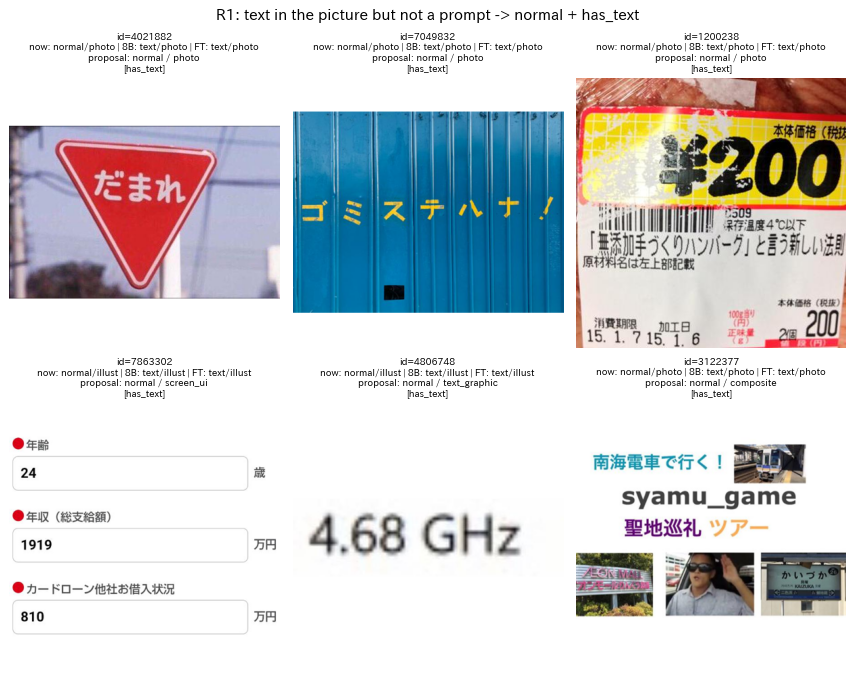
\includegraphics[width=\linewidth]{figures/fig_edge_text.png}
    \caption{文字を含むが回答者への問いではない画像の例}
    \label{fig_edge_text}
\end{figure}

標識，壁の文字，商品のラベル，入力フォームの画面は，目視では文章のお題ではないとして normal としたが，手法はいずれも text と予測した．
「画像の大部分が文章である」という見た目の基準では，これらの画像を text から除けない．
しかし，これらに必要なのは文章に答える処理ではなく，写真に一言を付ける通常の処理である．
以上から，約92\%の精度の上限は手法の差ではなくラベルの定義の曖昧さによって決まっていると判断し，ラベルの定義の見直しに進んだ．

\section{ラベルの定義の設計と改訂}
\label{sec_label}
本章では，初期の7クラスのラベルを，形式，属性，媒体の3軸のラベルに作り変えた経緯を述べる．
表\ref{tab_label_history}に，定義の改訂の要点をまとめる．

\begin{table*}[t]
    \centering
    \caption{ラベルの定義の改訂の経緯}
    \label{tab_label_history}
    \small
    \begin{tabular}{>{\raggedright\arraybackslash}p{0.12\textwidth}>{\raggedright\arraybackslash}p{0.5\textwidth}>{\raggedright\arraybackslash}p{0.3\textwidth}}
        \toprule
        版 & 主な内容 & 改訂の根拠 \\
        \midrule
        初期 & 形式4値と画風4値を統合した7クラス．text は「画像の大部分が文章」 & -- \\
        草案 & 形式（1つ），属性（複数），媒体（複数），事前知識（複数）の4軸 & 強い手法の誤りが定義の境界に集中 \\
        第1版 & 形式の優先順位，お題文の範囲，媒体の複数選択の制限，事前知識に作品不明を追加 & VLM による草案の試行で判断の揺れを確認 \\
        第2版 & テロップや字幕はお題文ではなく文字とする．事前知識の軸を廃止 & お題文と事前知識の判定が全手法で低精度 \\
        第3版 & 属性の合成画像を削除し，お題文ありとその他の文字ありを文字ありに統合．媒体の CG を削除 & 統合と削除の事後の分析と下流の処理での必要性 \\
        第4版 & 文字ありをロゴや透かしを含む読める文字全般に拡張．テンプレートの主題の文をお題文と明記 & 実データの目視による誤りの分析 \\
        \bottomrule
    \end{tabular}
\end{table*}

\subsection{定義の見直しの方針}
初期の定義には次の4つの問題があった．
第1に，定義が見た目に基づいており，ボケの生成に必要な処理と対応していなかった．
第2に，画風の軸に，絵の種類と事前知識の要否という2つの観点が混ざっていた．
例えば，ある作品のキャラクターを描いたイラストは，絵の種類はイラストであるが，ボケを作るには作品の知識が要る．
第3に，空欄を含む文章や空欄を含むカルタの札のように，複数の形式に当てはまる画像の優先順位が暗黙であった．
第4に，「大部分が」「主となる」のような程度の表現が，判断者によって異なる解釈を生んだ．

そこで，ラベルを使う下流の処理から逆算して定義を決める方針とした．
表\ref{tab_downstream}に，ボケの生成で必要となる処理と，その処理の要否を決めるラベルの対応を示す．
この対応に基づき，互いに排他的な形式と，同時に成り立ちうる属性を分け，画風の軸は画像の由来を表す媒体に限定した．

\begin{table}[t]
    \centering
    \caption{下流の処理とそれを決めるラベル}
    \label{tab_downstream}
    \small
    \begin{tabular}{>{\raggedright\arraybackslash}p{0.5\linewidth}>{\raggedright\arraybackslash}p{0.38\linewidth}}
        \toprule
        下流の処理 & ラベル \\
        \midrule
        お題文の読み取りと回答の生成 & 形式のお題文 \\
        空欄の位置の検出と語の生成 & 形式の穴埋め，空欄あり \\
        カルタの記号とひらがなの読み取り & 形式のカルタ，カルタ記号あり \\
        画像中の文字の読み取り & 文字あり \\
        作品の知識の参照 & 媒体のアニメ，マンガ，ゲーム，絵画 \\
        画風に応じた生成や分析 & 媒体 \\
        \bottomrule
    \end{tabular}
\end{table}

\subsection{4軸の草案と VLM による試行}
この方針から，形式，属性，媒体，事前知識の4軸からなる草案を作成した．
形式は回答の形を制限する性質であり，カルタ，穴埋め，お題文，通常から1つを選ぶ．
属性は空欄あり，お題文あり，カルタ記号あり，それ以外の文字ありの複数選択とした．
媒体は写真，アニメ，ゲーム，CG，マンガ，テキストグラフィック，絵画，イラストの複数選択とした．
事前知識は，実在の著名人を含むか，特定の作品に由来するものを含むかの複数選択とした．

草案の文言をそのまま Qwen3-VL-8B のプロンプトにし，通常の評価用データ640枚に適用した．
その結果，テキストグラフィックの定義である「文字が記入された画像」が広すぎ，54\%の画像で選ばれた．
媒体を2つ以上選んだ画像は46\%あり，アニメの画面に「アニメとイラスト」が付くように，1つの領域に複数の媒体が付いた．
お題文の定義の例示が問いと指示に限られていたため，「〜の共通点」「〜でありそうな事」のような題目の句や，状況を設定する文がお題文と判定されなかった．
また，空欄とお題文の両方がある29枚では，形式の判定が穴埋めとお題文に分かれた．

\subsection{ボケと投稿者の選択による裏付け}
草案では，形式は実際の大喜利とペアで決め，投稿者の意図をくみ取って判定するとした．
この方針がデータで裏付けられるかを，ボケの本文と \texttt{type} 列で確かめた．
カルタのお題には，記号のひらがなから始まるボケが集中するはずである．
そこで，お題 $ q $ に付いたボケのうち，かなで始まるものの最初の文字の分布から，書き出しの集中度 $ c_q $ を(\ref{eq_concentration})で定義した．

\begin{equation}
    c_q = \max_{s \in {\mathbb S}} \frac{|\{ b \in {\mathbb B}_q : {\rm first}(b) = s \}|}{|{\mathbb B}_q|}
    \label{eq_concentration}
\end{equation}

\noindent
ここで $ {\mathbb B}_q $ はお題 $ q $ に付いたボケのうちかなで始まるものの集合，$ {\mathbb S} $ はひらがなの集合，${\rm first}(b)$ はボケ $ b $ の括弧や記号を除いた最初の文字をひらがなに変換したものである．
漢字で始まるボケは読みが分からないため除いた．

図\ref{fig_boke_signals}の左に，目視の形式ごとの書き出しの集中度の分布を示す．
縦軸が集中度であり，かなで始まるボケが5件以上ある325枚を対象とした．
右は，ボケの文字数の中央値の分布である．

\begin{figure}[t]
    \centering
    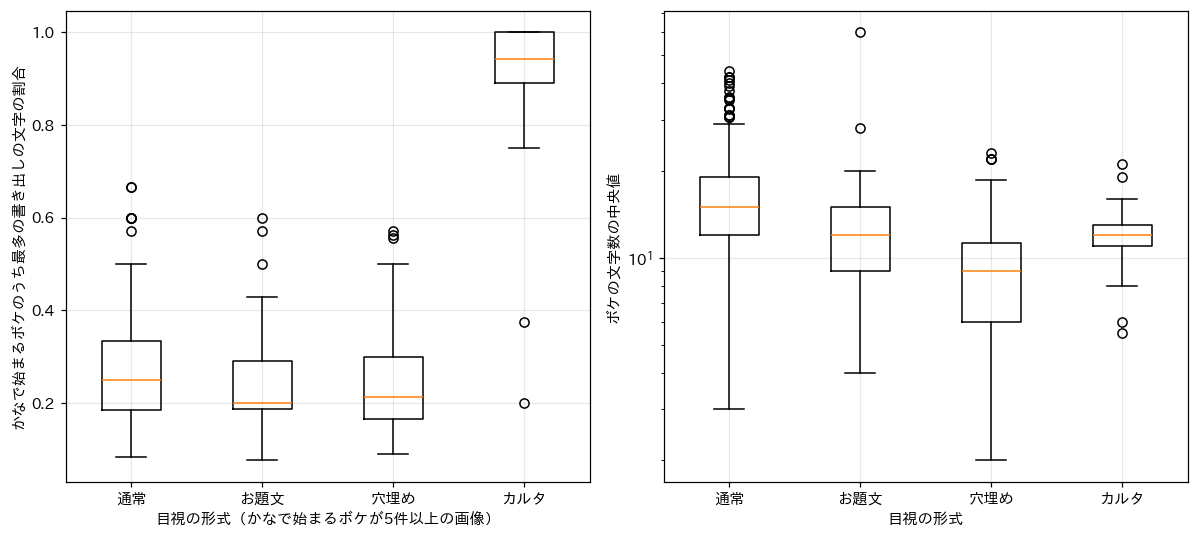
\includegraphics[width=\linewidth]{figures/fig_boke_signals.png}
    \caption{目視の形式ごとのボケの書き出しの集中度とボケの文字数の中央値}
    \label{fig_boke_signals}
\end{figure}

カルタの集中度の中央値は約0.94であり，他の形式の0.2から0.25と明確に分かれた．
集中度によるカルタの判別の AUC は 0.979 であった．
一方，ボケの文字数は形式ごとの分布の重なりが大きく，判別の手がかりとしては弱い．
\texttt{type} 列との照合では，\texttt{type} が穴埋めの52枚が全て目視でも穴埋めであり，文字の43枚のうち37枚が目視でお題文であった．
ただし，目視の穴埋めのうち \texttt{type} が穴埋めであったのは約74\%であり，投稿者の選択は適合率が高い一方で再現率は低い．
これらから，VLM の判定を主とし，ボケの書き出しと \texttt{type} 列を補助の証拠として用いる方針とした．

\subsection{第1版と第2版}
草案の試行の結果を受けて，第1版の定義を確定した．
形式は，カルタ，穴埋め，お題文，通常の順に判定し，最初に当てはまったものとする優先順位を明記した．
カルタの記号は文の一部ではなく独立した枠の中のひらがなに限り，穴埋めの空欄には黒塗りや話者に付いた空の吹き出しを含めた．
お題文には，問いと指示に加えて，題目の句，状況の設定，名前の列挙を含め，字幕や看板のように画像に元からある文字は含めないとした．
媒体は原則1つとし，複数選択は異なる媒体の領域が合成された画像に限った．
事前知識には，作品に由来するが作品名を特定できない場合を表す「作品不明」を加えた．

第1版で教師と生徒を評価したところ，事前知識の項目は教師を含む全手法で F1 が0.75未満であり，属性のお題文ありも F1 が約0.63にとどまった．
お題文ありの食い違いの多くは，テレビのテロップやアニメの字幕のように，投稿者が書き加えた文か元からある文字かを画像だけでは判別しにくいものであった．
そこで第2版では，テロップ，字幕，看板など投稿者が重畳したのではない文は，問いの形をしていてもお題文ではなく文字として扱い，テロップの中に空欄がある場合は穴埋めとした．
また，判断者の知識に依存し，教師の精度も低い事前知識の軸を廃止した．
この改訂により，教師のお題文ありの F1 は 0.63 から 0.79 に向上した．

\subsection{第3版：クラスの統合と削除}
第2版の段階で，教師と生徒の精度を下げている主な項目は，属性の合成画像，お題文ありとその他の文字ありの境界，媒体の CG であった．
クラスの統合や削除は，既存の予測と目視ラベルを同じ規則で読み替えれば，新たな学習なしに評価できる．
そこで，複数の統合と削除の案を事後に評価し，dev で選んで test で確かめた．
表\ref{tab_scheme}に，当時の最良の生徒における主な案の test のマクロ F1 を示す．

\begin{table}[t]
    \centering
    \caption{クラスの統合と削除の案の事後の評価（test のマクロ F1）}
    \label{tab_scheme}
    \small
    \begin{tabular}{llc}
        \toprule
        軸 & 案 & マクロ F1 \\
        \midrule
        \multirow{3}{*}{形式} & 現行の4クラス & 0.880 \\
         & お題文を通常に統合 & 0.923 \\
         & カルタを穴埋めに統合 & 0.884 \\
        \midrule
        \multirow{3}{*}{属性} & 現行の5項目 & 0.759 \\
         & 合成画像を削除 & 0.829 \\
         & 合成画像を削除し，文字を統合 & 0.911 \\
        \midrule
        \multirow{4}{*}{媒体} & 現行の8クラス & 0.826 \\
         & CG をイラストに統合 & 0.853 \\
         & CG と絵画をイラストに統合 & 0.877 \\
         & CG を削除 & 0.849 \\
        \bottomrule
    \end{tabular}
\end{table}

件数の少ないクラスを除けばマクロ F1 は機械的に上がるため，案の採否は精度だけでなく，表\ref{tab_downstream}の下流の処理での必要性からも判断した．
お題文を通常に統合する案は精度を最も上げたが，お題文は文字を読んで答える処理が必要な形式であり，区別が求められた種類そのものであるため採用しなかった．
合成画像は教師も生徒も F1 が0.42から0.51と最も低く，ボケの生成の処理も変えないため削除した．
お題文ありとその他の文字ありの誤りの多くは，テロップを投稿者が重畳した文とみなすかの判断にあった．
下流で必要なのは文字を読み取るかの判断のみであり，投稿者が書いた問いであるかは形式のお題文で既に表されている．
そこで2項目を文字ありに統合した．

媒体の CG は，目視で CG とした53枚のうち教師が CG と判定したのは21枚のみであり，残りは写真，ゲーム，イラスト，アニメに分散していた．
CG は，写実的な生成 AI の画像，3DCG のゲームやキャラクター，デジタルの絵にまたがっており，どのクラスに統合しても一部しか吸収できない．
そこで CG のクラス自体を削除し，3DCG や生成 AI の画像は，同じ見た目の画像を人が作った場合の媒体に振り分けることとした．
絵画をイラストに統合する案は数値では最も高かったが，絵画は F1 が0.72から0.76で判定できており，名画をもじった画像は元の作品の知識を要するため残した．
第3版で教師ラベルを付け直して生徒を学習したところ，生徒の test の3軸の平均は第2版の最良の 0.822 から 0.867〜0.897 に向上し，事後の分析による見込みの 0.880 とほぼ一致した．

\subsection{第4版：文字ありの範囲}
第3版の生徒で実データの無作為抽出160枚を確認したところ，誤りがあった41枚のうち18枚は文字ありのみの誤りであった．
そのうち17枚は，ロゴ，看板，ユニフォームの文字，画面の隅の小さな文字を，生徒が文字ありとしたものであった．
第3版の定義はロゴや透かしを除いていたが，教師はこれらを含めて回答しており，定義と教師の判定がずれていた．
文字ありの用途は，文字を手がかりにボケを分析する対象を絞ることであり，誤って含めても害は小さい．
そこで第4版では，ロゴ，透かし，著作権表示，衣服の文字なども含め，読める文字があれば文字ありとした．
文字が実際に大喜利に影響しているかは画像だけでは判断できないため，画像のラベルでは扱わず，ボケの文章を見る後段の処理で判断することとした．

さらに研究の最終段階で，ボケてのテンプレートや無地の背景に投稿者が書いた文が画像の主題である場合は，問いの形でなくてもお題文とすることを明記した．
台詞，題名，主張の文などであり，回答者はその文を読んで大喜利を作るためである．
ただし，ニュースの記事，ウェブやアプリの画面，テレビの字幕など，元からある文章を写したものは除く．

\subsection{最終の定義}
表\ref{tab_final_definition}に第4版の定義の要点を示す．
図\ref{fig_examples_final}に，最終の方法で無作為の20枚に付けたラベルを示す．
各画像の上に「形式｜属性｜媒体」の順でラベルを示し，属性の「空欄」は空欄あり，「文字」は文字あり，媒体の「テキスト」はテキストグラフィックを表す．
また，図\ref{fig_karuta_examples}にカルタの画像の例を示す．

\begin{table*}[t]
    \centering
    \caption{最終のラベルの定義（第4版）}
    \label{tab_final_definition}
    \small
    \begin{tabular}{>{\raggedright\arraybackslash}p{0.13\textwidth}>{\raggedright\arraybackslash}p{0.16\textwidth}>{\raggedright\arraybackslash}p{0.63\textwidth}}
        \toprule
        軸 & 項目 & 定義の要点 \\
        \midrule
        \multirow{4}{0.13\textwidth}{形式（1つ選択．上から順に判定）} & カルタ & ひらがな1文字が入った独立した記号がある．そのひらがなから始まる文を投稿する \\
         & 穴埋め & 語の代わりに置かれた空欄がある．○○，□，語の代わりの「？」，黒塗り，空の吹き出しを含み，顔の目隠しや文末の疑問符は含まない \\
         & お題文 & 投稿者が書き加えた，回答者に向けた問い，指示，題目の句，状況の設定，名前の列挙，テンプレートの主題の文がある．テロップ，字幕，看板など元からある文字は含まない \\
         & 通常 & 上記以外 \\
        \midrule
        \multirow{3}{0.13\textwidth}{属性（複数選択）} & 空欄あり & 穴埋めの空欄がある \\
         & カルタ記号あり & カルタの記号がある \\
         & 文字あり & ロゴ，透かし，衣服の文字を含め，読める文字がある．カルタ記号のひらがなのみの場合は除く \\
        \midrule
        \multirow{7}{0.13\textwidth}{媒体（原則1つ．合成画像では面積の約2割以上を占める各領域の媒体）} & 写真 & 現実の写真．実写の映像やフィギュアを撮影したものを含む \\
         & アニメ & アニメのスクリーンショット \\
         & ゲーム & ゲーム画面のキャプチャ \\
         & マンガ & 漫画作品から切り抜いたコマ．漫画風の一枚絵はイラスト \\
         & テキストグラフィック & 文字や記号が主体で，写真や絵がほとんどない画像 \\
         & 絵画 & 古典的な絵画．浮世絵などの版画と，写真に撮った絵画を含む \\
         & イラスト & 上記以外の絵．3DCG や生成 AI の画像は見た目に応じて振り分ける \\
        \bottomrule
    \end{tabular}
\end{table*}

\begin{figure*}[t]
    \centering
    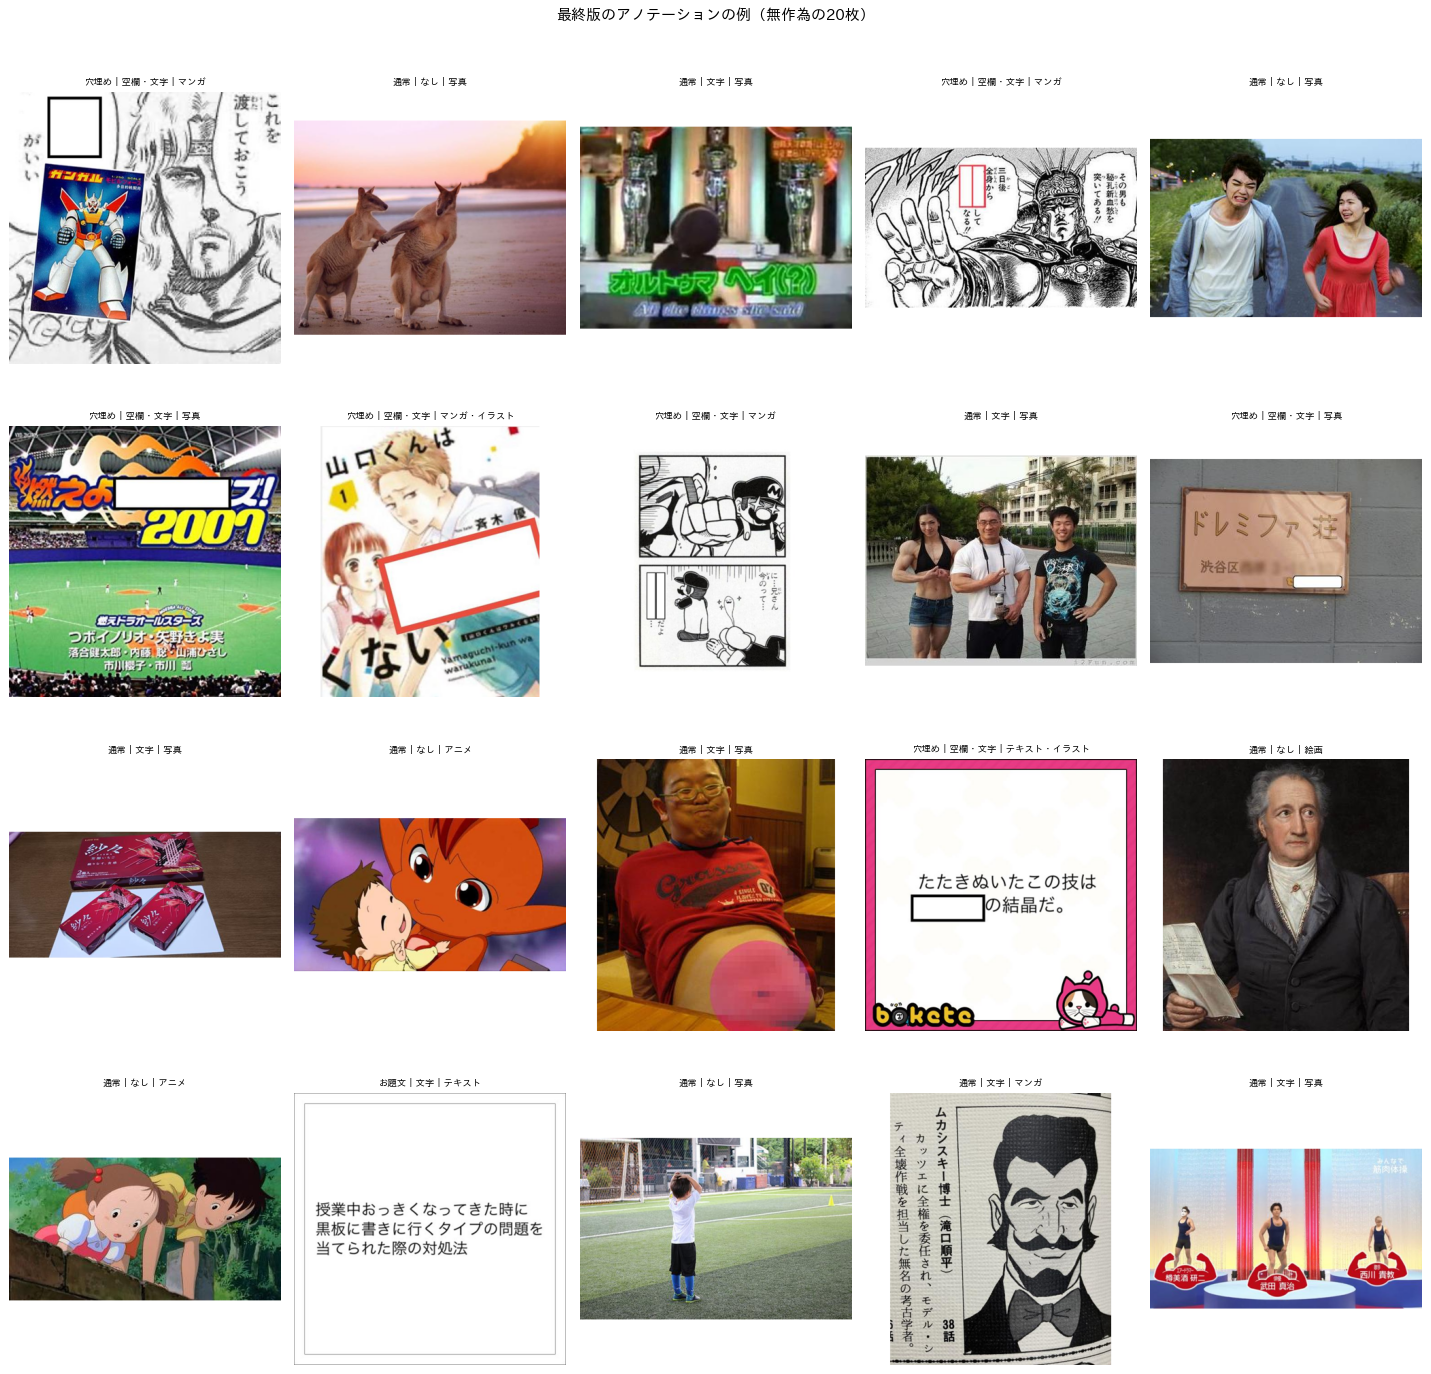
\includegraphics[width=0.85\textwidth]{figures/fig_examples_final.png}
    \caption{最終の方法によるアノテーションの例（無作為の20枚）}
    \label{fig_examples_final}
\end{figure*}

\begin{figure*}[t]
    \centering
    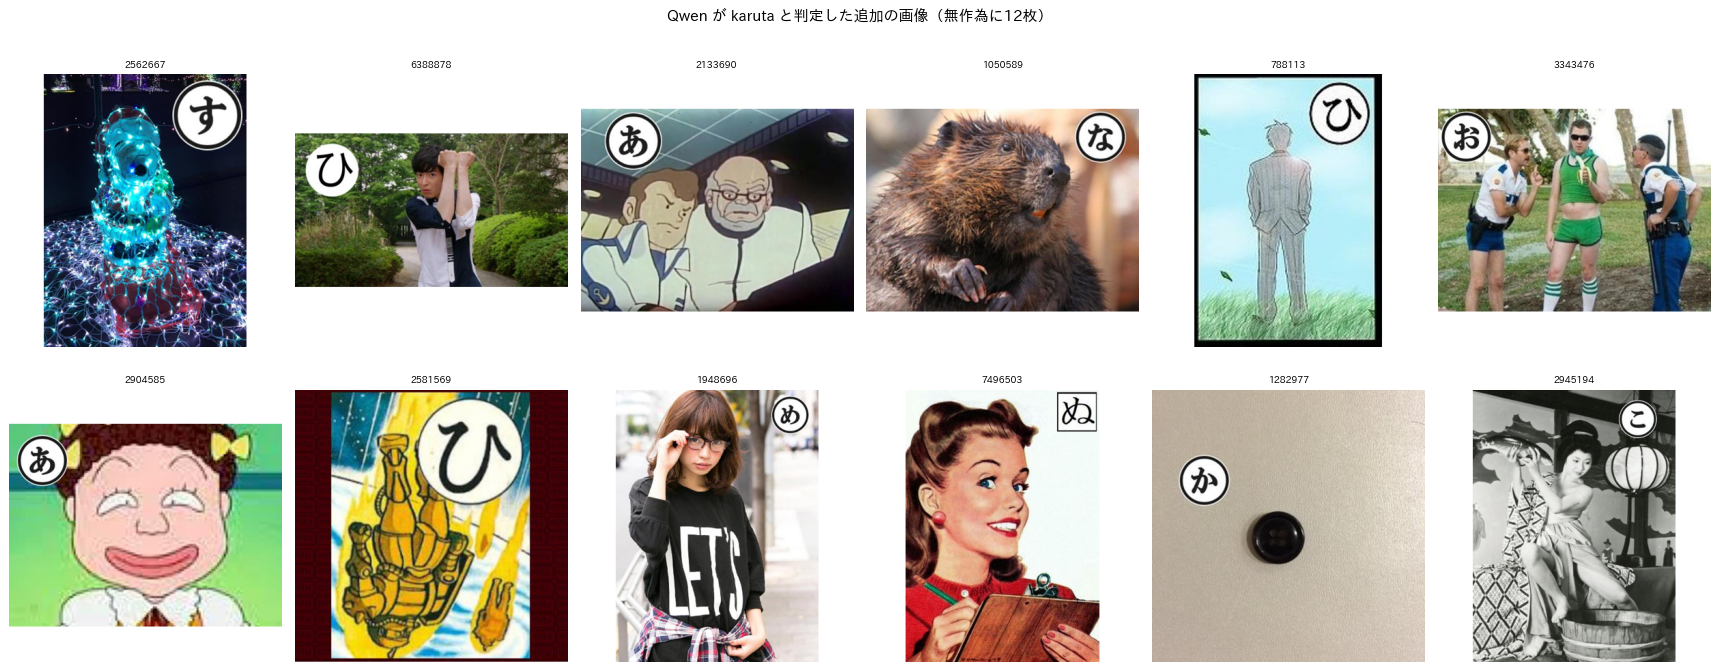
\includegraphics[width=0.9\textwidth]{figures/fig_karuta_examples.png}
    \caption{教師がカルタと判定した画像の例．画像の上の数字はお題 ID}
    \label{fig_karuta_examples}
\end{figure*}

\section{教師の構成}
\label{sec_teacher}
本章では，教師ラベルを付ける Qwen3-VL-8B への指示の方法を検討した結果を述べる．
以下では，VLM に与える指示文をプロンプトと呼び，1回の推論で1つのプロンプトを与えることを1つの質問と呼ぶ．
教師は，1枚の画像に複数の質問をし，その回答を規則で組み合わせる構成とした．

\subsection{推論の条件}
全ての質問は，Qwen3-VL-8B-Instruct を量子化せずに vLLM で実行した．
入力画像は1枚とし，最大画素数を $ 448 \times 448 $ に制限した．
生成は温度0の貪欲生成とし，出力は JSON スキーマによる構造化出力でラベルの候補に制約した．
入力の最大画素数を $ 256 \times 256 $ に下げると速度は約1.4倍になったが，正解率は 0.905 から 0.880 に低下した．
小さな空欄や文字の判読に解像度が必要なためと考えられる．
一方，$ 672 \times 672 $ に上げても形式の正解率の改善は0.6ポイントにとどまり，速度は半分になった．

\subsection{最終の教師の質問}
表\ref{tab_questions}に，最終の教師を構成する質問を示す．
表の名称は本稿での呼び名であり，括弧内は実装での識別子である．
実装の識別子は，プログラムと実験の記録との対応を示すために併記する．

\begin{table*}[t]
    \centering
    \caption{最終の教師を構成する質問}
    \label{tab_questions}
    \small
    \begin{tabular}{>{\raggedright\arraybackslash}p{0.2\textwidth}>{\raggedright\arraybackslash}p{0.42\textwidth}>{\raggedright\arraybackslash}p{0.3\textwidth}}
        \toprule
        質問の名称 & 内容 & 用い方 \\
        \midrule
        形式の質問（F\_v2） & 形式と画風を問う短い英語のプロンプト．text は「画像のほぼ全体が文章で，主となる写真や絵がない」と定義する & 形式の回答のみ用いる．text はお題文に読み替える \\
        お題文の確認（O\_v10\_en） & 投稿者が回答者に向けて書いた問い，指示，題目の句があるかを英語で問う & 形式の質問がお題文とした画像のみ．偽なら通常にする \\
        属性の質問（J\_v6） & 属性，形式，媒体を日本語で一括して問う．属性を先に出力させる & 属性の回答のみ用いる \\
        文字の質問（X\_v10\_en） & ロゴや透かしを含め，読める文字があるかを英語で問う & カルタ記号のない画像に限り，属性の質問の文字ありと論理和をとる \\
        媒体の質問（M\_v6） & 媒体のみを日本語で問う & CG の回答は削除し，媒体が空ならイラスト \\
        絵画の質問（P\_v8\_en） & 画家が描いた美術作品であるかを英語で問う & 媒体の絵画をこの回答で置き換える \\
        \bottomrule
    \end{tabular}
\end{table*}

回答を組み合わせた後に，次の規則を適用する．
第1に，形式から属性を導き，カルタならカルタ記号あり，穴埋めなら空欄あり，お題文なら文字ありとする．
第2に，媒体が1つも選ばれていない場合はイラストとする．
第3に，形式がカルタの画像は，ボケの書き出しで照合する．
かなで始まるボケが5件以上あり，そのうち VLM が読み取った記号のひらがなで始まる割合が3割未満であれば，カルタではないとみなす．
この規則は，空欄の前後のひらがなや中身が空の枠を，VLM がカルタの記号と誤る事例を減らすために導入し，教師のカルタの F1 を 0.77 から 0.88 に向上させた．

\subsection{質問の分け方}
表\ref{tab_split}に，質問の分け方を変えた教師の通常の評価用データ640枚での精度を示す．
1行目は事前知識を含む第1版の定義，それ以外は第2版の定義での値である．

\begin{table}[t]
    \centering
    \caption{質問の分け方と教師の精度（評価用データ640枚）}
    \label{tab_split}
    \small
    \begin{tabular}{>{\raggedright\arraybackslash}p{0.42\linewidth}ccc}
        \toprule
        構成 & 形式の正解率 & 属性 & 媒体 \\
        \midrule
        4軸を一括 & 0.850 & 0.707 & 0.769 \\
        3軸を一括 & 0.902 & 0.773 & 0.761 \\
        形式のみ分割 & 0.923 & 0.799 & 0.761 \\
        形式と媒体を分割 & 0.923 & 0.799 & 0.835 \\
        \bottomrule
    \end{tabular}
\end{table}

表\ref{tab_split}の属性と媒体の列はマクロ F1 である．
全ての軸を1つのプロンプトで問うと，出力が約150トークンに増え，個々の判断の精度が下がった．
形式は短いプロンプトで単独に問うと最も正確であり，媒体も媒体のみを問う方が一括で問うより高かった．
一方，属性は属性のみを問うより，形式と媒体の定義を含めて一括で問う方が高かった．
属性の判定には，形式の判定手順の文脈が役立つと考えられる．
質問を分けると推論の回数は増えるが，教師は数万枚にラベルを付けるのみであるため，全体の費用への影響は小さい．

\subsection{形式の質問の改訂の試み}
最も正確であった形式の質問は，初期の7クラスのために書いたプロンプトであり，text の定義は第2版以降のお題文の定義と一致しない．
そこで，定義を一致させる改訂を複数試みた．
表\ref{tab_format_prompt}に，dev における形式の正解率を示す．

\begin{table}[t]
    \centering
    \caption{形式の質問の改訂の試み（dev の形式の正解率）}
    \label{tab_format_prompt}
    \small
    \begin{tabular}{>{\raggedright\arraybackslash}p{0.7\linewidth}c}
        \toprule
        形式の質問 & 正解率 \\
        \midrule
        元の短い英語のプロンプト & 0.944 \\
        定義書の文言で書いた日本語のプロンプト & 0.894 \\
        同上，入力を $ 672 \times 672 $ 画素に拡大 & 0.900 \\
        同上，文字とその出所を先に書き出させる & 0.828 \\
        元のプロンプトの text を「絵があってもよい」に変更 & 0.487 \\
        同上，「多くの画像は該当しない」を追加 & 0.412 \\
        元のプロンプトに，テンプレートの問いの文の例を追加 & 0.881 \\
        \bottomrule
    \end{tabular}
\end{table}

いずれの改訂も元のプロンプトを超えなかった．
text の定義に「絵があってもよい」を加えると，標識や漫画の台詞だけでなく，文字のほとんどない人物の写真までお題文と判定した．
「画像のほぼ全体が文章」という見た目の基準は，定義書とは一致しないが VLM にとって判定しやすく，その基準を失うと判定の手がかりがなくなると考えられる．
画像中の文字とその出所を先に書き出させる方法も，途中の判断の誤りが形式の誤りにつながり，精度を下げた．
定義との不一致による実際の損失は，評価用データで2枚程度であったため，形式の質問は元のプロンプトを据え置いた．

\subsection{お題文の過検出への対策}
形式の質問の主な誤りは，看板，歌詞，報道の画面，図表など，画像に元からある文字が多い画像をお題文とする過検出であった．
この対策として，次の2通りを比較した．
1つ目は，形式の質問のお題文または通常の説明に「看板，字幕，歌詞，図表など元からある文字は大きくてもお題文ではない」を書き足す方法である．
2つ目は，形式の質問は変えず，お題文と判定した画像に限り，投稿者が回答者に向けて書いた文があるかを別の短い質問で確かめる方法である．
以下では，2つ目の質問を確認の質問と呼ぶ．

実データの目視ラベル380枚において，元の構成ではお題文の誤検出が13件であった．
説明をお題文の側に書き足すと誤検出は18件から19件に増え，通常の側に書き足すと10件に減った．
確認の質問を用いると誤検出は4件に減り，見落としは2件から3件に増えるのみであった．
教師のお題文の F1 は，実データで 0.769 から 0.873，通常の評価用データで 0.810 から 0.879 に向上した．
図\ref{fig_odaibun_verify}に，確認の質問でお題文から通常に戻した画像の例を示す．
各画像の上に，お題 ID と目視の形式を示す．
戻した32枚のうち27枚は目視でもお題文ではなく，看板，選挙のカード，歌詞，答案，報道の画面などであった．

\begin{figure*}[t]
    \centering
    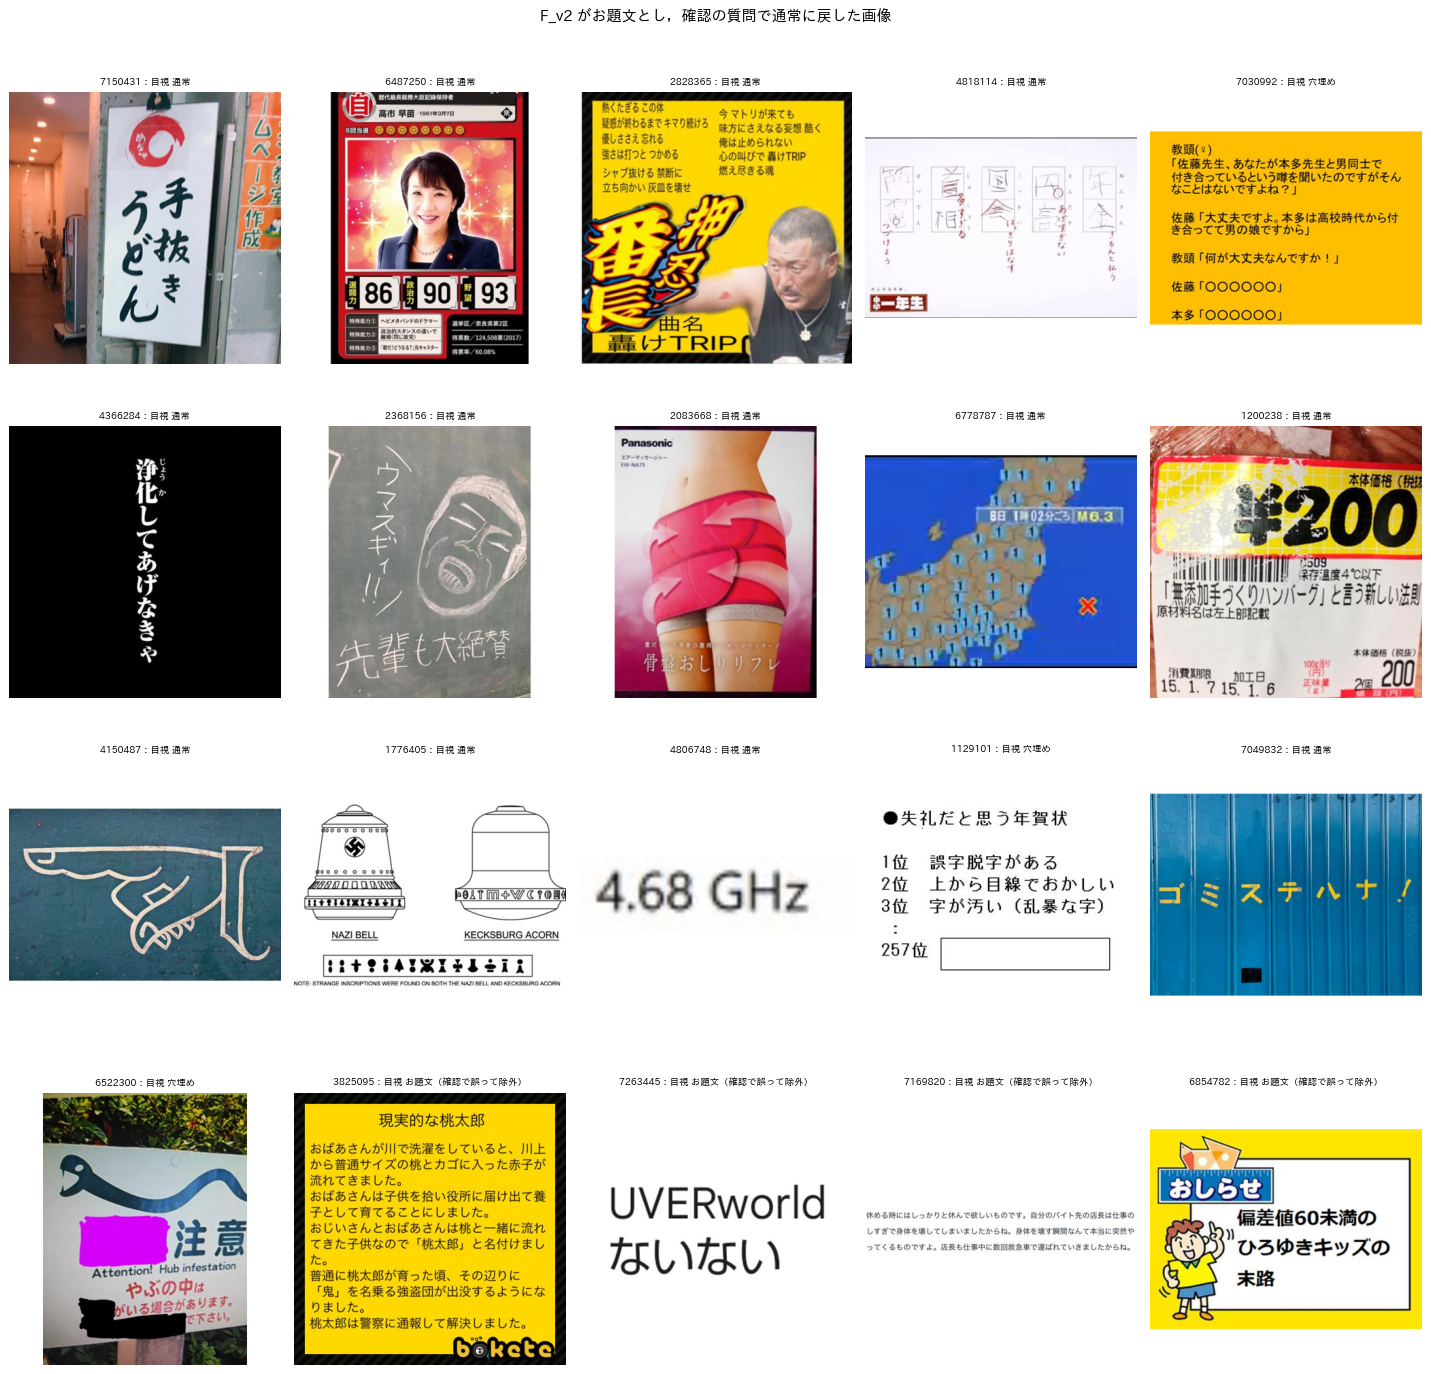
\includegraphics[width=0.8\textwidth]{figures/fig_odaibun_verify.png}
    \caption{形式の質問がお題文と判定し，確認の質問で通常に戻した画像の例}
    \label{fig_odaibun_verify}
\end{figure*}

同じ傾向は他の改訂でも見られた．
合成画像を「境界線で区切られた別々の写真の枚数」として問う質問や，お題文の位置と体裁を問う補助の質問は，いずれも適合率を下げた．
VLM は，テロップの帯やワイプの小窓を別々の写真と数え，テロップを投稿者が書き加えた文と判定した．
一方，絵画を独立の質問にすると，少ない区分の評価用データにおける教師の4区分の F1 の平均は，dev で 0.604 から 0.658，test で 0.591 から 0.715 に向上した．
媒体の質問では選択肢の多さに埋もれていた絵画が，独立の質問で見落とされにくくなったと考えられる．
これらの結果から，見た目で区別しにくい概念を問い方の工夫で判定させることは難しく，見た目の特徴がはっきりした概念や，誤りの多いクラスに対象を絞った確認の質問は有効であるといえる．

\subsection{文字ありの質問}
第4版の文字ありはロゴや透かしを含むが，属性の質問は旧定義に従ってこれらを除くよう指示していた．
そこで，読める文字があるかを独立に問う文字の質問を加えた．
文字の質問はほぼ見落としがない一方で，カルタの記号のひらがなだけの画像も文字ありと答えた．
そこで，カルタ記号のない画像に限り，文字の質問の回答と属性の質問の回答の論理和をとった．
これにより，教師の文字ありの F1 は実データで 0.954 から 0.971 に向上した．

\subsection{英語と日本語}
プロンプトの言語の影響を，属性の質問と絵画の質問で比較した．
英語版と日本語版のマクロ F1 の差は，いずれも0.001程度であった．
絵画の質問は，媒体の回答と組み合わせた場合に英語版が高かったため英語を採用し，他の質問は既存の言語のままとした．

\subsection{最終の教師の精度}
最終の教師は，通常の評価用データで dev の3軸の平均 0.916，test の3軸の平均 0.898 であり，実データの全項目一致の推定値は 0.803 であった．
教師ラベルは，全てのお題から無作為に抽出した40,000枚と，\ref{sec_student}章で述べる少ない区分の追加分の約5,000枚に付けた．
1枚あたり複数の質問をするため，教師の処理速度は毎秒約4から5枚であり，教師ラベルの付与には数時間を要した．

\section{生徒の構成}
\label{sec_student}
本章では，教師ラベルで学習する生徒の構成と，学習データの集め方および損失を検討した結果を述べる．

\subsection{生徒のモデル}
生徒には，埋め込みに対する MLP と，微調整した画像エンコーダの2種類を用いた．
MLP の入力は，SigLIP2-so400m の画像埋め込みを L2 正規化した1,152次元のベクトル $ {\mathbf x} \in {\mathbb R}^{1 \times 1152} $ である．
MLP の中間の表現 $ {\mathbf h} $ と，各軸の出力を(\ref{eq_mlp})に示す．

\begin{align}
    {\mathbf h} &= {\rm Dropout} \left( {\rm GELU} \left( {\rm LN}({\mathbf x}) {\mathbf W}_1 + {\mathbf b}_1 \right) \right),
    \nonumber \\
    {\mathbf p}^{\rm F} &= {\rm softmax} \left( {\mathbf h} {\mathbf W}_{\rm F} + {\mathbf b}_{\rm F} \right),
    \nonumber \\
    {\mathbf p}^{\rm A} &= \sigma \left( {\mathbf h} {\mathbf W}_{\rm A} + {\mathbf b}_{\rm A} \right),
    \quad
    {\mathbf p}^{\rm M} = \sigma \left( {\mathbf h} {\mathbf W}_{\rm M} + {\mathbf b}_{\rm M} \right)
    \label{eq_mlp}
\end{align}

\noindent
ここで ${\rm LN}$ は層正規化\cite{ref_layernorm}，${\rm GELU}$ は活性化関数\cite{ref_gelu}，${\rm Dropout}$ は確率0.3のドロップアウト\cite{ref_dropout}，$ \sigma $ は要素ごとのシグモイド関数である．
$ {\mathbf W}_1 \in {\mathbb R}^{1152 \times 1024} $ と $ {\mathbf b}_1 \in {\mathbb R}^{1 \times 1024} $ が中間層の重み行列としきい値ベクトルである．
$ {\mathbf W}_{\rm F}, {\mathbf W}_{\rm A}, {\mathbf W}_{\rm M} $ と $ {\mathbf b}_{\rm F}, {\mathbf b}_{\rm A}, {\mathbf b}_{\rm M} $ は，形式，属性，媒体の出力層の重み行列としきい値ベクトルである．
$ {\mathbf p}^{\rm F} \in {\mathbb R}^{1 \times 4} $ は形式の4クラスの確率，$ {\mathbf p}^{\rm A} \in {\mathbb R}^{1 \times 3} $ と $ {\mathbf p}^{\rm M} \in {\mathbb R}^{1 \times 7} $ は属性と媒体の各項目が真である確率である．
微調整のモデルは，SigLIP2-B の画像エンコーダの出力に，形式，属性，媒体の3つの線形の出力層を付けたものである．

学習の損失 $ L $ は，形式の交差エントロピーと，属性と媒体の各項目の2値交差エントロピーの和とし，(\ref{eq_loss})に示す．

\begin{align}
    L = &- \sum_{k=1}^{4} y^{\rm F}_k \log p^{\rm F}_k
    \nonumber \\
    &- \sum_{j \in {\mathbb J}} \left\{ y_j \log p_j + (1 - y_j) \log (1 - p_j) \right\}
    \label{eq_loss}
\end{align}

\noindent
ここで $ y^{\rm F}_k \in \{0, 1\} $ は教師ラベルの形式がクラス $ k $ であるかを表し，$ {\mathbb J} $ は属性と媒体の項目の集合，$ y_j \in \{0, 1\} $ と $ p_j $ は項目 $ j $ の教師ラベルと予測の確率である．
最適化には AdamW\cite{ref_adamw} を用いた．
MLP は学習率 $ 3 \times 10^{-4} $ で40エポック学習し，重み減衰は $ 10^{-4} $ と $ 10^{-2} $ から教師ラベルの検証用分割で選んだ．
微調整は，入力を $ 224 \times 224 $ 画素とし，学習率 $ 3 \times 10^{-5} $，重み減衰0.05，バッチサイズ128で5エポック学習した．
文字の向きを保つため左右反転の拡張は用いず，色の揺らぎのみを拡張とした．
いずれも検証用分割での3軸の平均が最良のエポックの重みを用いた．

予測では，形式は確率が最大のクラスとし，属性と媒体は確率0.5以上の項目を真とした．
媒体が1つも真でない場合は，確率が最大の媒体を真とした．
最後に，教師と同じ規則で形式から属性を導いた．

\subsection{少ない区分の追加}
無作為抽出の教師ラベル40,000枚では，CG が305枚，絵画が217枚，カルタが494枚しか含まれず，生徒はこれらをほとんど学習できなかった．
\ref{sec_selection}章では，少ない種類を多めに含む画像に教師ラベルを付ける方が効率が良いことを示した．
そこで，次の手順で少ない区分の画像を追加した．
まず，学習にも評価にも用いていない30万枚の候補に SigLIP2-so400m の埋め込みを計算した．
次に，40,000枚で学習した MLP で候補ごとに各区分の確率を求め，目標に達していない区分について確率の高い順に約1,000枚を選び，教師ラベルを付けた．
教師がその区分と判定した画像が40,000枚との合計で $ N_{\rm min} = 1{,}000 $ 枚以上になるまで，これを繰り返した．
以下では，40,000枚のみの学習データを基本の学習データ，追加分を含む学習データを追加ありの学習データと呼ぶ．

5回の繰り返しで計4,998枚を追加し，全区分が1,000枚以上になった．
最終的な枚数は，ゲーム1,715枚，CG 1,161枚，絵画1,075枚，カルタ1,178枚であった．
絵画は最も集まりにくく，2,666枚に教師ラベルを付ける必要があった．
追加のラベル付けは約30分で済んだ．

\subsection{重み付きの損失}
少ない区分の学習を強めるため，クラスの出現率に応じて重みを付けた損失も比較した．
形式のクラス $ k $ の交差エントロピーの重み $ v_k $ と，属性と媒体の項目 $ j $ の正例の重み $ u_j $ を(\ref{eq_weight})に示す．

\begin{equation}
    v_k \propto \left( \frac{N}{N_k} \right)^{\alpha},
    \qquad
    u_j = \left( \frac{N - P_j}{P_j} \right)^{\alpha}
    \label{eq_weight}
\end{equation}

\noindent
ここで $ N $ は学習データの枚数，$ N_k $ は教師ラベルの形式がクラス $ k $ である画像の数，$ P_j $ は項目 $ j $ の正例の数，$ \alpha = 0.5 $ である．
$ v_k $ は平均が1になるように正規化した．

表\ref{tab_rare_weight}に，第2版の定義における微調整した生徒の結果を示す．
少ない区分の F1 は，少ない区分の評価用データ第1版における4区分の F1 の平均である．

\begin{table}[t]
    \centering
    \caption{少ない区分の追加と重み付きの損失の効果（第2版の定義，微調整した SigLIP2-B）}
    \label{tab_rare_weight}
    \small
    \begin{tabular}{lccc}
        \toprule
        条件 & 少ない区分 & 3軸の平均 & 頑健な指標 \\
        \midrule
        基本，重みなし & 0.528 & 0.781 & 0.857 \\
        基本，重みあり & 0.676 & 0.803 & 0.847 \\
        追加あり，重みなし & 0.632 & 0.803 & 0.854 \\
        追加あり，重みあり & 0.713 & 0.812 & 0.845 \\
        \midrule
        教師 & 0.699 & 0.810 & 0.848 \\
        \bottomrule
    \end{tabular}
\end{table}

表\ref{tab_rare_weight}の3軸の平均と頑健な指標は，通常の評価用データの test での値である．
少ない区分の追加と重み付きの損失は，いずれも単独で少ない区分の F1 を上げ，併用すると教師と同等の 0.713 に達した．
改善は主に CG と絵画の再現率によるものであり，CG の F1 は 0.15 から 0.44，絵画は 0.08 から 0.51 に向上した．
一方，頑健な指標は 0.857 から 0.845 にわずかに下がり，重み付けは少ない区分の再現率を上げる代わりに多い区分の適合率を下げた．

ところが，第3版の定義で同じ比較を行うと，重み付きの損失は効果がなかった．
test の媒体のマクロ F1 は，重みを付けると全ての条件で下がり，例えば追加ありの学習データで 0.896 から 0.840 に低下した．
また，媒体を2つ以上選ぶ画像の割合が，実データで6\%から7\%程度から8\%から11\%に増え，目視ラベルの6.3\%から離れた．
第2版で重みが有効であったのは，境界の曖昧な CG のような少ない区分があったためと考えられる．
そこで第3版以降では重み付きの損失を廃止し，少ない区分の追加のみを用いた．

\subsection{生徒のモデルの比較と確率の平均}
最終の教師ラベルで，生徒のモデルとその組み合わせを比較した．
組み合わせでは，複数のモデルの確率を(\ref{eq_ensemble})のように平均した．

\begin{equation}
    \bar{\mathbf p} = \frac{1}{M} \sum_{m=1}^{M} {\mathbf p}^{(m)}
    \label{eq_ensemble}
\end{equation}

\noindent
ここで $ M $ は組み合わせるモデルの数，$ {\mathbf p}^{(m)} $ は $ m $ 番目のモデルが出力した形式，属性，媒体の確率を連結したベクトルである．
予測の規則は，平均した確率 $ \bar{\mathbf p} $ に適用する．

選択の指標は，通常の評価用データの dev の3軸の平均と，少ない区分の評価用データの dev の4区分の F1 の平均の平均とした．
test と実データの目視ラベルは確認のみに用いた．
表\ref{tab_student_models}に主な結果を示す．
単体のモデルは3つの乱数の種の平均であり，「MLP 3種」は3つの乱数の種で学習した MLP の確率の平均である．

\begin{table*}[t]
    \centering
    \caption{生徒のモデルの比較（最終の教師ラベル）}
    \label{tab_student_models}
    \footnotesize
    \begin{tabular}{lcccccc}
        \toprule
        モデル & 選択の指標 & dev 3軸 & 少ない区分 test & test 3軸 & 全項目一致 & 枚/秒 \\
        \midrule
        MLP 3種 ＋ 微調整 SigLIP2-B 224画素 & {\bf 0.872} & 0.919 & 0.888 & 0.919 & 0.838 & 約150 \\
        MLP ＋ 微調整 SigLIP2-B 224画素 ＋ 384画素 & 0.863 & 0.925 & 0.862 & 0.914 & 0.838 & 約115 \\
        MLP ＋ 微調整 SigLIP2-B 224画素 & 0.860 & 0.915 & 0.889 & 0.925 & 0.846 & 約150 \\
        MLP ＋ 微調整 SigLIP2-B 384画素 & 0.858 & 0.924 & 0.856 & 0.920 & 0.837 & 約135 \\
        MLP（単体） & 0.847 & 0.900 & 0.845 & 0.889 & 0.797 & 約180 \\
        微調整 SigLIP2-B 224画素（単体） & 0.836 & 0.905 & 0.839 & 0.896 & 0.795 & 約750 \\
        微調整 SigLIP2-B 384画素（単体） & 0.825 & 0.911 & 0.824 & 0.896 & 0.806 & 約410 \\
        \bottomrule
    \end{tabular}
\end{table*}

最も効果が大きかったのは，MLP と微調整のモデルの確率の平均であった．
実データの全項目一致の推定値は，単体の約0.80から約0.84に，少ない区分の test は0.84から0.89に向上した．
MLP は少ない区分に強く，微調整のモデルは通常の画像の形式と文字に強いため，誤りの傾向が異なる2つのモデルの平均が互いの弱点を補ったと考えられる．
入力を384画素にした微調整は，単体では dev が高いものの少ない区分の F1 が低く，組み合わせても224画素を上回らなかった．
MLP は埋め込みを共有するため，3つの乱数の種を平均しても計算量はほとんど増えない．
以上から，選択の指標が最良であった「MLP 3種と224画素の微調整 SigLIP2-B の確率の平均」を最終の生徒とした．

\section{最終の構成と精度}
\label{sec_final}
\subsection{処理の流れ}
図\ref{fig_pipeline}に，最終のアノテーションの処理の流れを示す．
処理は，画像の列挙，生徒による予測，お題文の確認，ラベルの決定の4段階からなる．

\begin{figure}[t]
    \centering
    \begin{tikzpicture}[
        node distance=4mm,
        box/.style={draw, rounded corners=2pt, align=center, font=\footnotesize, minimum width=0.86\linewidth, inner sep=3pt},
        arr/.style={-{Stealth[length=2mm]}, thick}
    ]
        \node[box] (list) {1. 列挙：ハッシュ値が同じ画像をまとめる \\ 6,823,270件 $\to$ 6,609,511枚};
        \node[box, below=of list] (pred) {2. 予測：SigLIP2-so400m の埋め込み $\to$ MLP 3種 \\ ＋ 微調整した SigLIP2-B の確率の平均};
        \node[box, below=of pred] (ver) {3. 確認：お題文と予測した約8\%の画像に \\ Qwen3-VL-8B で確認の質問};
        \node[box, below=of ver] (fin) {4. 決定：確認で偽ならお題文以外で最大の形式 \\ 形式から属性を導き，お題ごとに保存};
        \draw[arr] (list) -- (pred);
        \draw[arr] (pred) -- (ver);
        \draw[arr] (ver) -- (fin);
    \end{tikzpicture}
    \caption{最終のアノテーションの処理の流れ}
    \label{fig_pipeline}
\end{figure}

列挙の段階では，ハッシュ値が同じ画像のうち代表の1枚のみを予測し，結果を同じ内容の全てのお題に展開する．
予測の段階では，各画像を1回だけ読み込み，SigLIP2-so400m の埋め込みと微調整した SigLIP2-B の確率を同時に求める．
埋め込みは保存しておき，ラベルの定義を見直す場合に，教師ラベルを付け直して MLP を学習し直すだけで全件のラベルを更新できるようにした．
確認の段階では，平均した確率で形式がお題文となった画像に限り，Qwen3-VL-8B に確認の質問をする．
決定の段階では，確認の質問の回答が偽の画像を，お題文以外で確率が最大の形式に変え，形式から属性を導く．

\subsection{確認の質問の選択}
教師の構成では，お題文の確認に表\ref{tab_questions}の確認の質問を用いた．
最終の構成の生徒は，2つのモデルの確率の平均によってお題文の誤検出が既に少なく，評価用データでは確認の質問の有無による差がほとんどなかった．
そこで，学習にも評価にも用いていない無作為の2万枚に全ての段階を適用し，確認の質問の働きを直接確かめた．

生徒がお題文と予測した1,615枚のうち，教師と同じ確認の質問はお題文ではないと145枚を答えた．
この145枚を目視で確認したところ，98枚は実際にはお題文であった．
図\ref{fig_o10_wrong}に例を示す．
その多くは，ボケてのテンプレートに投稿者が書いた「こんな〜は嫌だ」のような典型的な題目の句や，主題となる台詞の文であった．
評価用データにはこの種の画像が少ないため，評価用データだけではこの欠点が見えなかった．

\begin{figure*}[t]
    \centering
    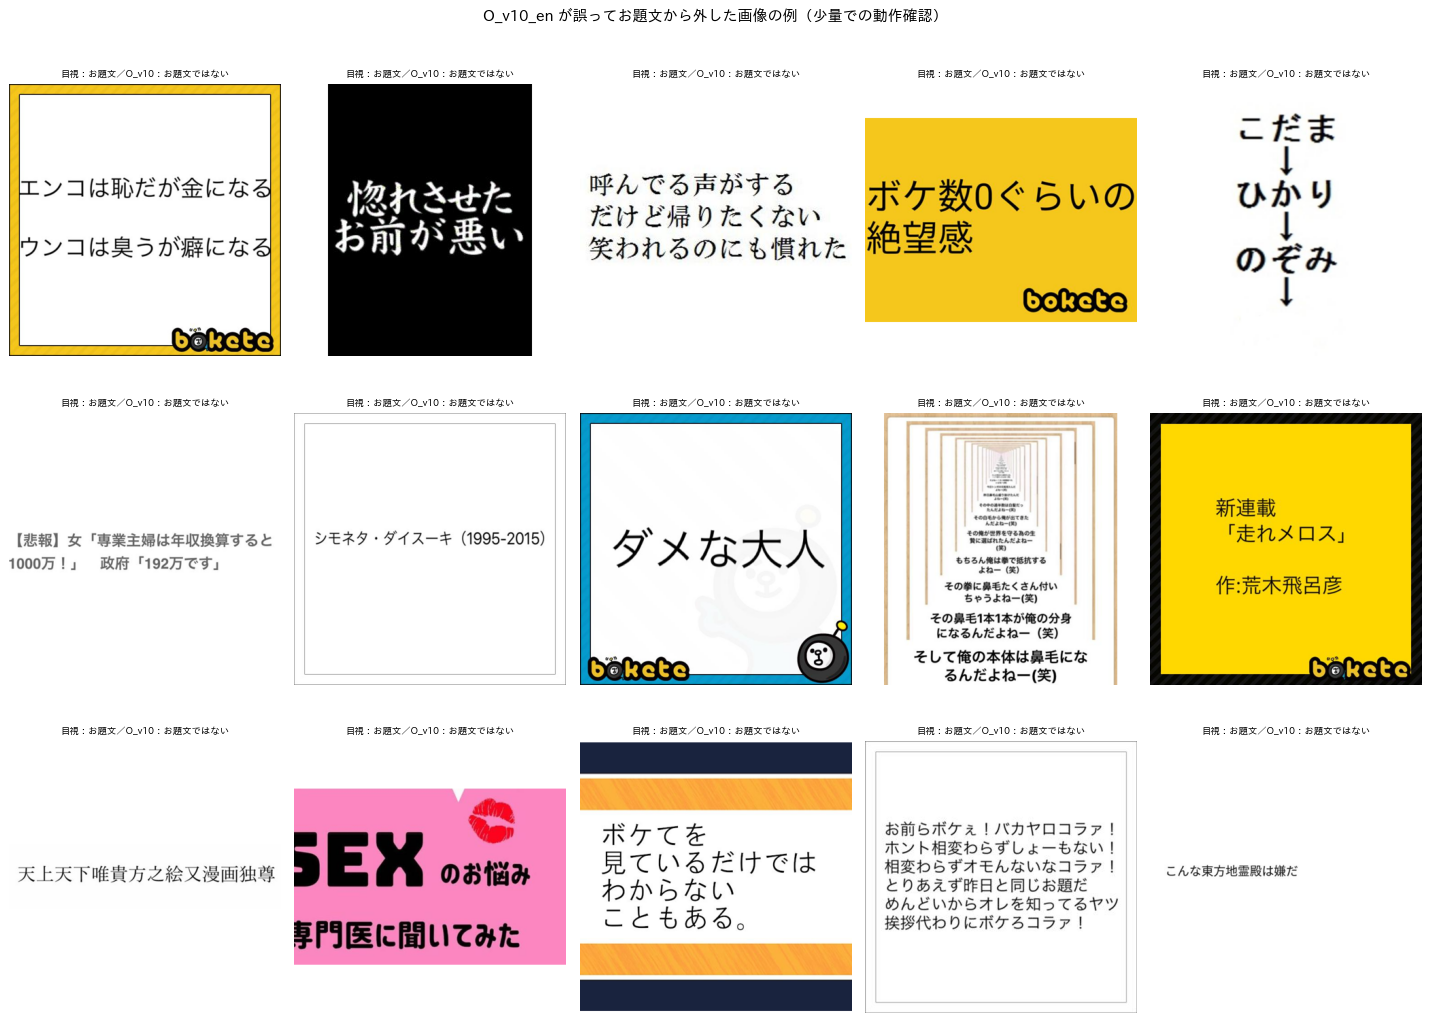
\includegraphics[width=0.8\textwidth]{figures/fig_o10_wrong.png}
    \caption{教師の構成の確認の質問が誤ってお題文から外した画像の例．画像の上に目視の形式と確認の質問の回答を示す}
    \label{fig_o10_wrong}
\end{figure*}

そこで，題目の句の典型的な型と，テンプレートや無地の背景に書かれた主題の文を真とする例として明示し，看板，報道の画面，ウェブの記事，歌詞，ゲームや漫画の台詞など文字が全て元の素材から来ている場合を偽とする例として明示した確認の質問を作成した．
実装の識別子は O\_v11\_en である．
この質問がお題文ではないと答えたのは9枚であり，アプリのエラー画面，ゲームの画面，報道の画面，看板などで，全て正しかった．
効果は全データの約0.05\%と小さいが，誤りは見つからなかったため，最終の構成ではこの質問を用いた．

なお，教師ラベルをこの質問で作り直した場合も比較したが，その教師ラベルで学習した生徒はお題文と予測する割合が実データで9.5\%と高くなり，全ての評価で劣った．
そのため，教師ラベルは表\ref{tab_questions}の構成のままとした．
ボケの書き出しによるカルタの取り消しも比較したが，生徒の予測では評価用データ全体で1枚しか変わらず，その1枚は正しいカルタであったため用いなかった．
教師ではこの規則がカルタの誤検出を減らしたが，生徒はカルタの誤検出が既に少ないためである．

\subsection{最終の構成の精度}
表\ref{tab_final_items}に，最終の構成の項目ごとの F1 を示す．
test は通常の評価用データの最終評価用の320枚，層別は実データの層別抽出の220枚での値，推定は(\ref{eq_ipw})による実際の分布での推定値である．

\begin{table}[t]
    \centering
    \caption{最終の構成の項目ごとの F1}
    \label{tab_final_items}
    \small
    \begin{tabular}{llccc}
        \toprule
        軸 & 項目 & test & 層別 & 推定 \\
        \midrule
        \multirow{4}{*}{形式} & カルタ & 0.88 & 1.00 & 1.00 \\
         & 穴埋め & 0.93 & 0.98 & 0.94 \\
         & お題文 & 0.89 & 0.86 & 0.87 \\
         & 通常 & 0.96 & 0.97 & 0.97 \\
        \midrule
        \multirow{2}{*}{属性} & 空欄あり & 0.94 & 0.98 & 0.95 \\
         & 文字あり & 0.97 & 0.97 & 0.97 \\
        \midrule
        \multirow{7}{*}{媒体} & 写真 & 0.97 & 0.96 & 0.98 \\
         & アニメ & 0.89 & 0.96 & 0.88 \\
         & ゲーム & 0.89 & 0.91 & 0.90 \\
         & マンガ & 0.91 & 0.98 & 0.99 \\
         & テキストグラフィック & 0.95 & 0.90 & 0.92 \\
         & 絵画 & 1.00 & 0.79 & 0.46 \\
         & イラスト & 0.78 & 0.73 & 0.82 \\
        \bottomrule
    \end{tabular}
\end{table}

最終の構成は，通常の評価用データの test で3軸の平均 0.919，少ない区分の評価用データの test でゲーム，絵画，カルタの F1 の平均 0.888，実データの全項目一致の推定値 0.838 を達成した．
埋め込みの MLP 単体では，それぞれ 0.886，0.845，0.797 であった．
test のゲームは5枚，絵画は3枚のみであり，F1 の値は不安定である．
絵画の推定値 0.46 も，実データの目視ラベルに絵画が15枚しかなく，重みの大きい1枚から2枚の誤りで大きく動く．
絵画の精度は，少ない区分の評価用データでの F1 0.84 で見るのが適切である．
最も低い項目はイラストであり，アニメ風の一枚絵，ゲームの絵，絵本の挿絵との境界が曖昧で，目視でも判断が分かれた．

\subsection{精度の推移}
表\ref{tab_progress}に，研究の各段階の代表的な構成の精度を示す．
定義が変わると評価用ラベルも付け直しているため，異なる段階の数値は厳密には比較できないが，段階ごとの改善の傾向を示す．

\begin{table}[t]
    \centering
    \caption{研究の各段階の代表的な生徒の精度}
    \label{tab_progress}
    \small
    \begin{tabular}{>{\raggedright\arraybackslash}p{0.5\linewidth}>{\raggedright\arraybackslash}p{0.38\linewidth}}
        \toprule
        段階と生徒 & 精度 \\
        \midrule
        初期の7クラス，線形プローブ & 正解率 0.913 \\
        第1版の4軸，MLP & 4軸の平均 0.778 \\
        第2版の3軸，微調整，追加ありと重み & test の3軸の平均 0.812 \\
        第2版，絵画の質問を加えた教師，MLP & test の3軸の平均 0.822 \\
        第3版，MLP，追加あり & test の3軸の平均 0.897 \\
        第4版，MLP，追加あり & 全項目一致の推定値 0.802 \\
        第4版，最終の構成 & test の3軸の平均 0.919，全項目一致の推定値 0.838 \\
        \bottomrule
    \end{tabular}
\end{table}

\subsection{処理時間}
予測の段階は，GPU での SigLIP2-so400m の計算が律速であり，画像の読み込みのプロセス数を増やしても速度は GPU のみの速度である毎秒約205枚に近い値にとどまった．
無作為の2万枚での予測の速度は毎秒約150枚，確認の質問の速度は毎秒約22枚であった．
処理時間を優先する場合は，確認の質問を省くと全項目一致の推定値をほぼ保ったまま確認の段階を省け，微調整した SigLIP2-B のみを用いると全件を約2.5時間で処理できるが，全項目一致の推定値は 0.795 に下がる．

\section{全データへの適用}
\label{sec_full}
\subsection{処理の実績}
最終の構成を BoketeDBv4 の全てのお題画像に適用した．
予測の段階では，6,609,511枚の代表画像を36,634秒，すなわち約10.2時間で処理し，速度は毎秒約180枚であった．
無作為の2万枚での測定より速いのは，画像の読み込みのプロセス数を増やしたためである．
確認の質問の対象は，形式がお題文と予測された551,260枚であり，代表画像の8.3\%であった．
本稿の執筆の時点で，確認の段階は対象のうち320,000枚を処理しており，速度は毎秒約33枚であった．
この速度では，確認の段階の全体に約4.7時間を要する．
したがって，以下に示す全データの集計は，確認の質問を適用する前の予測による．
確認の質問で形式が変わる画像は，無作為の2万枚で約0.05\%であったため，以下の集計への影響は小さいと見込まれる．

\subsection{ラベルの分布}
表\ref{tab_full_dist}に，全6,823,270件のお題におけるラベルの割合を示す．
比較のため，実データの無作為抽出160枚の目視ラベルの割合も示す．

\begin{table}[t]
    \centering
    \caption{全データにおけるラベルの割合（確認の質問の前の予測）}
    \label{tab_full_dist}
    \small
    \begin{tabular}{llcc}
        \toprule
        軸 & 項目 & 全データ & 目視（160枚） \\
        \midrule
        \multirow{4}{*}{形式} & カルタ & 1.1\% & 1.9\% \\
         & 穴埋め & 20.1\% & 19.4\% \\
         & お題文 & 8.3\% & 6.9\% \\
         & 通常 & 70.5\% & 71.9\% \\
        \midrule
        \multirow{3}{*}{属性} & 空欄あり & 21.4\% & -- \\
         & カルタ記号あり & 1.1\% & -- \\
         & 文字あり & 58.6\% & 60.6\% \\
        \midrule
        \multirow{7}{*}{媒体} & 写真 & 53.1\% & 53.7\% \\
         & アニメ & 9.1\% & 8.1\% \\
         & ゲーム & 2.3\% & 2.5\% \\
         & マンガ & 15.2\% & 16.3\% \\
         & テキストグラフィック & 14.5\% & 14.4\% \\
         & 絵画 & 0.9\% & 0.0\% \\
         & イラスト & 11.2\% & 10.6\% \\
        \midrule
        \multicolumn{2}{l}{媒体を2つ以上選んだ画像} & 6.0\% & 6.3\% \\
        \bottomrule
    \end{tabular}
\end{table}

全データの分布は，160枚の目視ラベルの分布とおおむね一致した．
お題の約3割は通常以外の形式であり，そのうち穴埋めが約2割と最も多い．
お題文は目視ラベルよりやや高く，これは確認の質問の前の予測であることと，\ref{sec_final}章で示したお題文の適合率の限界による．
媒体では，写真が約半数を占め，作品の知識を前提としうるアニメ，マンガ，ゲーム，絵画の割合の合計は，複数選択を重複して数えて約28\%であった．
文字ありは約59\%であり，画像の過半数に何らかの読める文字が含まれる．

\subsection{投稿年ごとの推移}
図\ref{fig_full_year_format}に，投稿年ごとの通常以外の形式の割合を示す．
横軸はお題の投稿年，縦軸はその年に投稿されたお題に占める割合である．
2026年はデータの収集の時点までの値である．

\begin{figure}[t]
    \centering
    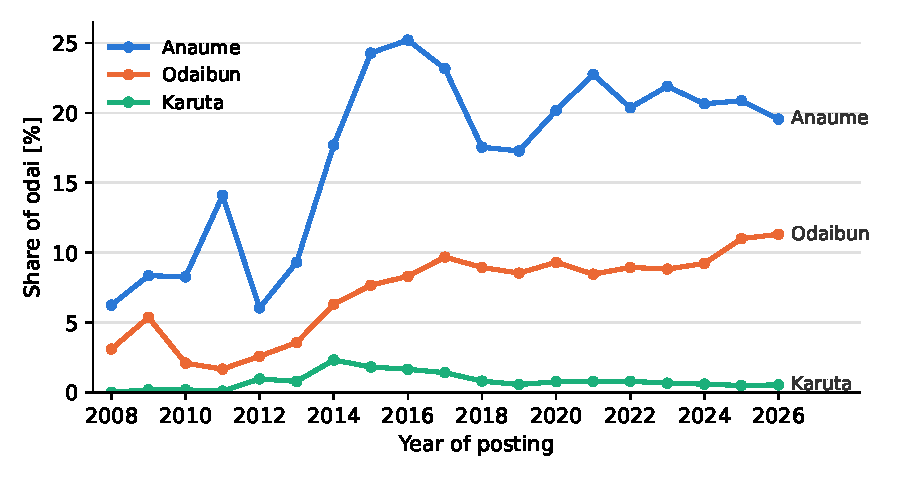
\includegraphics[width=\linewidth]{figures/fig_full_year_format.pdf}
    \caption{投稿年ごとの形式の割合．Anaume は穴埋め，Odaibun はお題文，Karuta はカルタを表す}
    \label{fig_full_year_format}
\end{figure}

穴埋めの割合は2013年以前は6\%から14\%であったが，2014年から急増し，2016年に25.2\%で最大となった．
その後は17\%から23\%で推移している．
お題文の割合は2013年以前は2\%から5\%であったが，その後は徐々に増え，2025年以降は約11\%となった．
カルタは2014年の2.3\%が最大であり，近年は1\%未満である．
2008年から2012年は年間のお題数が2万件から10万件程度と少なく，割合の変動が大きい．

図\ref{fig_full_year_media}に，投稿年ごとの媒体と文字ありの割合を示す．
各図の横軸は投稿年，縦軸はその年のお題に占める割合であり，縦軸の範囲は図ごとに異なる．

\begin{figure*}[t]
    \centering
    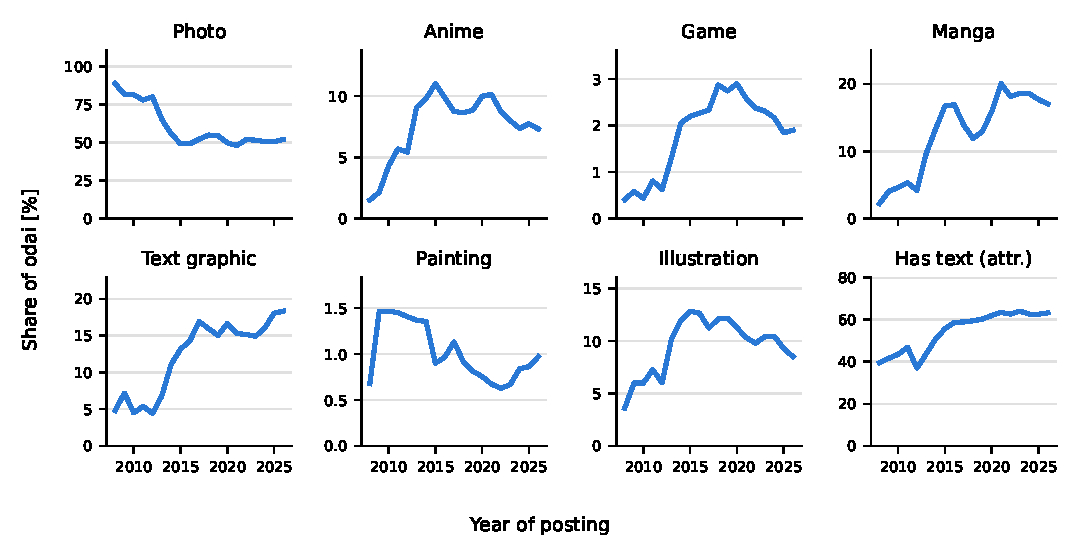
\includegraphics[width=0.85\textwidth]{figures/fig_full_year_media.pdf}
    \caption{投稿年ごとの媒体と文字ありの割合．Photo は写真，Anime はアニメ，Game はゲーム，Manga はマンガ，Text graphic はテキストグラフィック，Painting は絵画，Illustration はイラスト，Has text は属性の文字ありを表す}
    \label{fig_full_year_media}
\end{figure*}

写真の割合は2008年の約89\%から2015年の約49\%まで下がり，その後は約50\%で推移している．
代わりに，アニメ，マンガ，テキストグラフィック，イラストの割合が2013年から2015年にかけて増えた．
文字ありの割合も約40\%から約60\%に増えており，お題画像は写真に一言を付けるものから，文字や作品の画像を用いるものへと多様化したといえる．
ただし，これらの推移は生徒の予測に基づくものであり，年ごとの精度の違いは評価していない．

\section{考察}
\label{sec_discussion}
\subsection{精度を決めた要因}
研究の全体を通じて，精度を最も大きく変えたのはモデルの選択ではなく，ラベルの質とラベルの定義であった．
初期の比較では，同じ SigLIP2-so400m の埋め込みでも，メタデータの弱いラベルで学習すると正解率は約0.70，VLM のラベルで学習すると0.91であった．
VLM 自体も，プロンプトの定義を明確にするだけで正解率が約19ポイント向上したのに対し，8B から32B へのモデルの大型化では向上しなかった．
また，第2版から第3版への定義の改訂では，生徒の構成を変えずに test の3軸の平均が約0.07向上した．

ラベルの定義を改訂する際に有効であったのは，下流の処理から逆算する考え方と，判断が揃わない区別を無理に残さない判断である．
事前知識，合成画像，CG は，いずれも研究上の関心はあるが，判断者の知識や境界の解釈に依存し，教師と目視の判定が揃わなかった．
これらを廃止または統合した結果，残ったクラスはいずれも見た目で判定でき，かつ下流の処理と1対1に対応するものになった．
一方で，お題文と通常の境界は，形式の誤りの大半を占めるにもかかわらず，お題文の読み取りという処理に直結するため維持した．
精度のためにクラスを統合すると，マクロ F1 は機械的に上がるため，統合の判断は精度だけでなく用途に基づいて行う必要がある．

\subsection{VLM への指示の方法}
VLM への指示では，質問を分ける，対象を絞って別の短い質問で確かめるという方法が有効であり，説明を書き足す，思考の過程を書き出させるという方法は有効でなかった．
説明を書き足すと，Qwen3-VL-8B はかえって説明の対象のクラスを選びやすくなった．
また，見た目で区別しにくい概念を問い方の工夫で判定させる試みは，合成画像やお題文の体裁の質問のように，いずれも失敗した．
これらの結果は，VLM による分類のプロンプトは短く見た目に基づく基準で書き，判定の難しい部分は対象を絞った別の質問に切り出す方が安定することを示唆する．
ただし，これらの比較は Qwen3-VL-8B のみで行っており，他のモデルで同じ傾向が成り立つかは確かめていない．

\subsection{評価用データの重要性}
研究の過程では，評価用データで有効に見えた方法が，実データでは問題を起こす事例が2度あった．
1つ目は，媒体の定義を具体化したプロンプトであり，dev では媒体のマクロ F1 を 0.773 から 0.858 に上げたが，test では 0.859 から 0.760 に下げた．
差の大部分は各3枚以下の CG と絵画の正誤によるものであり，件数の少ない項目でプロンプトを調整すると偶然の正誤に引きずられる．
2つ目は，教師の構成の確認の質問であり，評価用データでは有効であったが，無作為の2万枚では典型的なお題文の多くを誤って外していた．
評価用データに典型的なテンプレートの画像が少なかったことが原因である．
これらの経験から，評価用データを dev と test に分けることに加え，少ない区分を多く含む評価用データと，実データの無作為抽出による確認を併用することが重要であるといえる．
層別抽出と抽出確率の逆数による重み付けは，少ないクラスの件数を確保しつつ実際の分布での精度を推定する方法として有用であった．

\subsection{限界}
本研究には次の限界がある．
第1に，全ての目視ラベルは1名の判断者によるものであり，判断者間の一致度を測っていない．
目視ラベルは，画像を表示して内容を確認できる AI エージェントが付与したものであり，人の判断者によるラベルとの一致は確かめていない．
特に，イラストとアニメやゲームの境界，テンプレートの文をお題文とするか，面積の約2割の領域に媒体を付けるかの判断には揺れが残る．
第2に，教師のプロンプトの多くは通常の評価用データの誤りを見て改訂したため，教師の精度は楽観的である．
生徒の構成の選択は dev で行い test で報告したが，プロンプトの選択の一部には test の結果も参照した段階がある．
第3に，絵画やゲームのような少ないクラスは，実データの目視ラベルでの件数が少なく，推定値の誤差が大きい．
第4に，評価用データの文字ありの見直しは，いずれかのモデルが文字ありと予測した画像に限ったため，全てのモデルが見落とした小さな文字が残っている可能性がある．
第5に，全データの集計は確認の質問の前の予測によるものであり，年ごとの精度の違いは評価していない．

\section{おわりに}
\label{sec_conclusion}
本稿では，大喜利投稿サイト「ボケて」の約682万件のお題画像に，大喜利の形式，画像中の記号や文字の有無，画像の媒体を表すラベルを，有料の API を用いずに単一の GPU で付与する方法を確立するまでの経緯と分析を報告した．
VLM である Qwen3-VL-8B を教師とし，SigLIP 2 に基づく分類器を生徒とする蒸留は，教師と同等以上の精度を約1桁速い速度で得た．
精度の上限はラベルの定義の曖昧さによって決まっており，ボケの生成に必要な処理から逆算してラベルの定義を4回改訂することで，判定の揃うラベルの体系を得た．
教師の構成では，軸ごとに質問を分け，誤りの多いお題文に限って別の短い質問で確かめる方法が有効であった．
生徒の構成では，生徒の予測で少ない区分を選んで教師ラベルを追加する方法と，埋め込みの MLP と微調整した画像エンコーダの確率を平均する方法が有効であった．
最終の構成は，評価用データで3軸のマクロ F1 の平均 0.919，実データで全項目一致の推定値 0.838 を達成し，全データの予測を約10.2時間で完了した．
全データの集計から，穴埋めがお題の約2割を占めること，2014年前後を境にお題画像が写真中心から文字や作品の画像を含むものへと多様化したことが分かった．

今後の課題として，複数の人の判断者による目視ラベルの一致度の測定，確認の質問を適用した後の全データの無作為抽出による精度の確認，穴埋めの空欄の位置とカルタのひらがなの検出の定量評価が挙げられる．
また，属性の文字ありが大喜利の回答に実際に影響しているかを，ボケの文章を用いて判定する後段の処理の構築も課題である．


\vspace{-1mm}
\begin{thebibliography}{99}

    \bibitem{ref_bokete}
    ボケて (bokete), https://bokete.jp/, (2026年10月閲覧).

    \bibitem{ref_clip}
    A. Radford, et al., ``Learning Transferable Visual Models From Natural Language Supervision,'' Proc. ICML, 2021.

    \bibitem{ref_siglip}
    X. Zhai, B. Mustafa, A. Kolesnikov, and L. Beyer, ``Sigmoid Loss for Language Image Pre-Training,'' Proc. ICCV, 2023.

    \bibitem{ref_siglip2}
    M. Tschannen, et al., ``SigLIP 2: Multilingual Vision-Language Encoders with Improved Semantic Understanding, Localization, and Dense Features,'' arXiv:2502.14786, 2025.

    \bibitem{ref_qwen3vl}
    Qwen Team, ``Qwen3-VL Technical Report,'' arXiv:2511.21631, 2025.

    \bibitem{ref_internvl35}
    W. Wang, et al., ``InternVL3.5: Advancing Open-Source Multimodal Models in Versatility, Reasoning, and Efficiency,'' arXiv:2508.18265, 2025.

    \bibitem{ref_minicpmv}
    Y. Yao, et al., ``MiniCPM-V: A GPT-4V Level MLLM on Your Phone,'' arXiv:2408.01800, 2024.

    \bibitem{ref_vllm}
    W. Kwon, et al., ``Efficient Memory Management for Large Language Model Serving with PagedAttention,'' Proc. SOSP, 2023.

    \bibitem{ref_kd}
    G. Hinton, O. Vinyals, and J. Dean, ``Distilling the Knowledge in a Neural Network,'' arXiv:1503.02531, 2015.

    \bibitem{ref_convnext}
    Z. Liu, et al., ``A ConvNet for the 2020s,'' Proc. CVPR, 2022.

    \bibitem{ref_yomitoku}
    K. Kinoshita, ``YomiToku: AI-OCR for Japanese documents,'' https://github.com/kotaro-kinoshita/yomitoku, 2024.

    \bibitem{ref_layernorm}
    J. L. Ba, J. R. Kiros, and G. E. Hinton, ``Layer Normalization,'' arXiv:1607.06450, 2016.

    \bibitem{ref_gelu}
    D. Hendrycks and K. Gimpel, ``Gaussian Error Linear Units (GELUs),'' arXiv:1606.08415, 2016.

    \bibitem{ref_dropout}
    N. Srivastava, et al., ``Dropout: A Simple Way to Prevent Neural Networks from Overfitting,'' JMLR, vol. 15, pp. 1929--1958, 2014.

    \bibitem{ref_adamw}
    I. Loshchilov and F. Hutter, ``Decoupled Weight Decay Regularization,'' Proc. ICLR, 2019.

\end{thebibliography}


\end{document}
